\section{The Standard Model}
This section is primarily based on quantum field theory undergraduate lecture notes from Tim Evans \cite{timevans}, David Tong \cite{tong} and lecture notes on unification by Arttu Rajantie.

The standard model (SM) is the best description of fundamental physics at the quantum scale. It is a \textit{quantum field theory} (QFT) that describes the interactions of the fundamental particles, which emerge as quantised excitations of fields. In order to understand the details of this theory, one must first be introduced to the concepts of quantum mechanics and classical field theory.

\subsection{Quantum Mechanics and Classical Field Theory}

The equations of motion of a classical system are determined by the \textit{principle of least action}. This states that the trajectory $x(t)$ of a particle is the one that extremises the \textit{action} $S$:
\begin{equation}
    S=\int\mathrm{d}t L(x,\dot{x}),
\end{equation}
where $L(x,\dot{x})$ is called the \textit{Lagrangian}. In this \textit{Lagrangian formulism}, a particle trajectory is parametrised by its coordinates $x$ and their time derivative $\dot{x}$.

In the equivalent Hamiltonian formalism of classical physics, a point particle is parametrised by coordinates and momenta $(x,p)$. A function called the Hamiltonian ($H$) is defined which describes the evolution in the space of coordinates and momenta, called \textit{phase space}. The equations of motion are given by Hamilton's equations:
\begin{equation}\label{eq:hameq}
    %\dot{x_i}=\frac{\partial H}{\partial p_i},\hspace{10pt}\dot{p_i}=-\frac{\partial H}{\partial q_i}\hspace{10pt}
    \dot{x}=\{x,H\},\hspace{10pt}\dot{p}=\{p,H\},
\end{equation}
where $\{,\}$ are the Poisson brackets, and a dot denotes the partial derivative with time. The Poisson brackets for coordinates and momenta are:
\begin{equation}\label{eq:coordpois}
    \{x,p\}=1, \hspace{5pt} \{x,x\} =0, \hspace{5pt} \{p,p\}=0,
\end{equation}
and the time evolution of any function $F(x,t)$ can be expressed in terms of the Poisson brackets:
\begin{equation}\label{eq:operatorevo}
    \frac{\mathrm{d}F}{\mathrm{d}t}=\{F,H\}.
\end{equation}
The probability of being in $\mathrm{d}p\mathrm{d}x$ is denoted through a probability density function $w(p,x,t)$:
\begin{equation}\label{eq:probdens}
    w(p,x,t)\mathrm{d}p\mathrm{d}x,\hspace{2pt}\text{where}\hspace{2pt} \int\mathrm{d}p\mathrm{d}x\hspace{2pt}w(p,x,t)=1.
\end{equation}
Quantum Mechanics (QM) can be defined through the direct quantisation of a classical dynamical system of particles, in a process known as canonical quantisation. In this process, the system is \textit{quantised} by replacing Poisson bracket relations with a commutator relation times $i/\hbar$, and replacing the conjugate variables $x,p$ with operators $\hat{x},\hat{p}$. For a finite system of point particles, the canonical commutation relations are written as:
\begin{equation}
    [\hat{x_i},\hat{p_j}] = i \hbar\delta_{ij}, \hspace{5pt} [\hat{x}_i,\hat{x}_j]=[\hat{p}_i,\hat{p}_j]=0.
\end{equation}
There are many interpretations of quantum mechanics, one of the most used ones is the \textit{Copenhagen Interpretation}, which proposes that the state of the system is described analogously to equation \ref{eq:probdens} by a \textit{wave function}, $\psi(\mathbf{x})$, where the probability density $p(\mathbf{x})$ of finding the system in a given state is described by the \textit{Born rule}:
\begin{equation}\label{eq:bornrule}
    p(\mathbf{x})\mathrm{d}^3x=|\psi|^2\mathrm{d}^3x,\hspace{2pt}\text{where} \int\mathrm{d}^3x\hspace{2pt}|\psi(\mathbf{x})|^2=1.
\end{equation}
This description of reality has a number of problems. First, the universe is assumed to be split into quantum and classical regimes, where classical physics emerges at larger scales (lower energies). Secondly, QM only describes a finite number single-particle states -- this can be seen from equation \ref{eq:bornrule}, which states that a particle exists with probability 1. This is problematic since this is at odds with the principle of matter-energy equivalence from special relativity. Namely, single-particle states don't allow for the creation of particle-antiparticle pairs. Additionally, a multi-particle theory is necessary from the standpoint of causality. This is less obvious, but a good description of causality violation is given in \cite{Theory:PeskinSchroeder}.

In classical field theory, single particle states are replaced by a \textit{fields} which are functions defined at every point in space and time. This formalism describes the dynamics of continuous systems with an infinite number of degrees of freedom. Examples of classical fields are the electric and magnetic fields in Maxwell's theory of electromagnetism. The equations of motion are again determined through the principle of least action, where the Lagrangian is replaced by its continuous generalisation, the \textit{Lagrangian density}, $\mathcal{L}$ -- in the rest of this chapter $\mathcal{L}$ will simply be referred to as the Lagrangian. The action is written as:
\begin{equation}
    S=\int\mathrm{d}^4x \mathcal{L}(\phi,\partial_\mu\phi),
\end{equation}
where the index $\mu$ runs over one time coordinate $(x^0)$ and three space coordinates $(x^1,x^2,x^3)$ and $\partial_\mu\equiv\frac{\partial}{\partial x^\mu}$. One of the most important aspects of a field theory is the invariance of the action under a set of symmetries. If a given transformation leaves the laws of physics unchanged, the Lagrangian must be left unchanged up to a total derivative. In particular, a relativistic field theory requires that the Lagrangian is invariant under Lorentz transformations. Fields which transform under the trivial representation of the Lorentz group (the value of the field at any spacetime point remains unchanged) are called \textit{scalar fields}\footnote{In the SM, scalar fields are spin-zero fields, and their excitations represent Bosons.}. These fields don't come with a \textit{Lorentz index}, $\mu$. Fields with a Lorentz index are called \textit{vector fields}, and the components of these fields change under non-trivial Lorentz transformations. The Lagrangian can also have \textit{internal symmetries}, which specifies the invariance of the theory under some symmetry group. Demanding a number of internal symmetries, limits the form of $\mathcal{L}$, and therefore limits the theory by, for example, only allowing certain interactions.

To introduce QFT, it is useful to start with the simple classical field theory of a real, non-interacting scalar field. After enforcing the theory to be invariant under the group of spacetime symmetries (Poincare group), the only possible Lagrangian is of the form:
\begin{equation}\label{eq:kg}
    \lag=\frac{1}{2}(\dmu\phi)^2-\frac{1}{2}m^2\phi^2.
\end{equation}
This corresponds to the equations of motion:
\begin{equation}\label{eq:kgeom}
    \ddmu\phi+m^2\phi=0,
\end{equation}
which is the Klein-Gordon equation, and describes a relativistic spin-zero field of mass $m$. This field theory can be quantised in a similar procedure to the canonical quantisation. This is done by promoting the field and its conjugate momentum-density $\pi(x)\equiv\frac{\partial\lag}{\partial\dot{\phi}}$ to operators and enforcing the axioms:
\begin{equation}
    [\hat{\phi}(\mathbf{x},t),\hat{\pi}(\mathbf{y},t)]=i\hbar\delta^{(3)}(\mathbf{x}-\mathbf{y}), \hspace{15pt} [\hat{\phi}(\mathbf{x},t),\hat{\phi}(\mathbf{y},t)]=[\hat{\pi}(\mathbf{x},t),\hat{\pi}(\mathbf{y},t)]=0,
\end{equation}
where $\delta^{(3)}(\mathbf{x}-\mathbf{y})$ is the Kronecker delta function. These are called the \textit{equal time commutation relations}. In going from QM to QFT, the coordinates $\mathbf{x}$ no longer represent quantised operators, but are arguments of the field. This is a big conceptual shift -- fields represent deviations in a \textit{field space}. This is very different to QM, where the equations of motion describe the dynamics of single particles in coordinate space.

\subsection{Quantum Electrodynamics (QED)}

Maxwell's theory of electrodynamics can be described as a classical field theory using the \textit{scalar potential} $\phi$ and the \textit{vector potential} $\mathbf{A}$. The electric and magnetic fields are given in terms of the potentials by:
\begin{equation}
    \mathbf{E}=-\frac{\partial\mathbf{A}}{\partial t}-\mathbf{\nabla}\phi,\hspace{25pt}\mathbf{B}=\mathbf{\nabla}\times\mathbf{A}.
\end{equation}
These scalar and vector potentials can be combined into a real Lorentz vector field, the \textit{four-vector potential} $A^\mu=(\phi,\mathbf{A})$. 

Let's assume the Lagrangian of classical electrodynamics involves $A^\mu$ and its derivative $\dmu\anu$. The general form of the Lagrangian can be derived from the knowledge that $\lag$ must be (i) a Lorentz scalar, (ii) \textit{renormalisable}, and (iii) invariant under \textit{gauge transformations}. Renormalisation is a concept from QFT which limits the energy dimensions of the terms in the Lagrangian. Namely, renormalisable terms are those with energy dimensions of at most 4, since the introduction of higher dimension terms leads to divergent cross-sections. Gauge invariance is simply the statement that certain changes to the scalar and vector potentials $\phi$ and $\mathbf{A}$ leave the electric field $\mathbf{E}$ and the magnetic field $\mathbf{B}$ invariant. These gauge transformations are given by:
\begin{equation}
   \amu\rightarrow\amu-\dmu\lambda(x)
\end{equation}
where $\lambda$ is an arbitrary scalar function. It is immediately clear that terms like $\amu A^\mu$ and $\dmu A^\mu$ are not invariant under gauge transformations, and are therefore not allowed. The only renormalisable Lorentz scalar term which is invariant under gauge transformations is:
\begin{equation}\label{eq:maxwell}
    \lag=-\frac{1}{4}F_{\mu\nu}F^{\mu\nu},
\end{equation}
where \fmunu is the anti-symmetric tensor known as the \textit{field strength tensor} $\fmunu=\dmu\anu-\dnu\amu$, and the normalisation of $-\frac{1}{4}$ is chosen by convention. The equations of motion corresponding to this Lagrangian reproduce all of Maxwell's equations but with no charge-density and current-density terms. This describes the dynamics of massless, non-interacting spin-1 fields, which can be identified as photons in the quantised theory. 

Scalar and vector fields give rise to spin-0 and spin-1 particles, respectively. To describe leptons and quarks, which have spin-1/2, requires the concept of \textit{spinor} fields $\psi$. The Lagrangian which describes the dynamics of fermions in the SM is given by the Dirac Lagrangian:
\begin{equation}\label{eq:dirac}
    \lag=\bar{\psi}(i\gamma^\mu\dmu-m)\psi,
\end{equation}
where $\gamma^{\mu}$ are the gamma matrices, which are a set of four $4\times4$ matrices which satisfy the \textit{Clifford Algebra}, and $\bar{\psi}\equiv\psi^\dagger\gamma^0$. The equations of motion are given by the Dirac equation:
\begin{equation}
    i(\slashed{\partial}-m)\psi=0,
\end{equation}
where a slash indicates contraction with the gamma matrices. The Dirac equation is a first-order equation which replaces the Klein-Gordon equation for spin-1/2 particles. The plane-wave solutions to the Dirac equation represent particles and antiparticles with energies given by $E^2=\mathbf{p}^2+m^2$.

The Dirac Lagrangian has a global\footnote{A \textit{global} symmetry transformation is not position-dependent, whereas a \textit{local} symmetry transformation is position-dependent.} U(1) symmetry, i.e. it is invariant under the transformation $\psi\rightarrow e^{i\theta}\psi$. As a consequence of Noether's theorem, which states that every continuous symmetry of the action has a corresponding conservation law, this symmetry results in a conserved \textit{current}, $j^\mu$, which satisfies the continuity equation. This gives rise to an associated conserved \textit{charge}. The current is given by:
\begin{equation}\label{eq:current}
    j^\mu=-e\bar{\psi}\gamma^\mu\psi, \hspace{5pt}\text{where}\hspace{5pt} \dmu j^\mu=0,
\end{equation} 
where $-e$ is the charge of the electron. In the quantised Dirac theory, this gives rise to the conserved charge given by:
\begin{equation}
    Q=\int-e\sum_s(\hat{N}{}_a^s-\hat{N}{}_b^s)\frac{d^3p}{(2\pi)^3},
\end{equation}
where $\hat{N}{}_a^s$ and $\hat{N}{}_b^s$ are the number operators for fermions and anti-fermions, respectively, in spin state $s$. The global U(1) symmetry of the Dirac Lagrangian therefore gives rise to particle number, and as a consequence, electric charge conservation \cite{Theory:PeskinSchroeder}.  

The description of QED given by the Dirac Lagrangian (\ref{eq:dirac}) and the Maxwell Lagrangian (\ref{eq:maxwell}) does not give the full picture. First, the Maxwell term does not reproduce Maxwell's equations for non-zero electric charge, and there is still no description of interactions between photons and fermions. Both of these issues are solved by adding an extra interaction term, $-j^\mu A_\mu$, where $j^\mu$ is the conserved current in equation \ref{eq:current}. With this additional term, the QED Lagrangian is given by:
\begin{equation}
    \lag=-\frac{1}{4}F_{\mu\nu}F^{\mu\nu} + \bar{\psi}(i\slashed{\partial}-m)\psi + e\bar{\psi}\gamma^\mu\psi\amu.
\end{equation}
This is equivalent to:
\begin{equation}\label{eq:qed}
    -\frac{1}{4}F_{\mu\nu}F^{\mu\nu} + \bar{\psi}(i\slashed{D}-m)\psi, \hspace{5pt}\text{where}\hspace{5pt} D_\mu\equiv\dmu+ie\amu.
\end{equation}
$D_\mu$ is referred to as the \textit{covariant derivative}. In going from the sum of the Maxwell (Equation \ref{eq:maxwell}) and Dirac Lagrangians (Equation \ref{eq:dirac}) to Equation \ref{eq:qed}, a global U(1) symmetry is replaced by a local U(1) symmetry. This process of turning a global symmetry into a local symmetry through the introduction of the covariant derivative has given rise to interactions between fields.

The Dirac Lagrangian (Equation \ref{eq:dirac}) is invariant under parity transformations defined by $(t,\mathbf{x})\rightarrow(t,-\mathbf{x})$ if the spinor as transforms as $\psi\rightarrow\gamma^0\psi$. However, this contradicts experimental observations of parity violation in beta decay \cite{Theory:parityviolation}. The generalisation of \textit{Dirac spinors} to left- and right-handed \textit{Weyl spinors} allows parity to be violated. By introducing a fifth gamma matrix $\gamma^5$ which anti-commutes with all other gamma matrices, Hermitian ``Left'' and ``Right'' projection operators can be defined
\begin{equation}
    P_L=\frac{1}{2}(\mathds{1}-\gamma^5),\hspace{10pt}P_R=\frac{1}{2}(\mathds{1}+\gamma^5),
\end{equation}
which are then used to construct the Weyl spinors
\begin{equation}
    \psi_L=P_L\psi,\hspace{10pt}\psi_R=P_R\psi,\hspace{5pt}\text{where}\hspace{5pt}\psi=\psi_L+\psi_R.
\end{equation}
It can be shown that left (right) handed Weyl spinors transform into left (right) handed Weyl spinors under Lorentz transformations, which implies it's possible to construct a Lorentz invariant theory using Weyl spinors. Under parity transformations, however, left-handed Weyl spinors turn into right-handed Weyl spinors, and vice-versa, giving rise to parity violating theories. The Dirac Lagrangian (Equation \ref{eq:dirac}) can be written in terms of Weyl spinors as
\begin{equation}\label{eq:weyllag}
    \lag=\bar{\psi}_Li\slashed{\partial}\psi_L+\bar{\psi}_Ri\slashed{\partial}\psi_R-m(\bar{\psi}_L\psi_R+\bar{\psi}_R\psi_L),
\end{equation}
where the spinors decouple at $m=0$. The handed-ness is interpreted as the helicity of the particle, i.e. whether the spin is parallel or anti-parallel to the momentum. This is only well-defined in the $m=0$ case as here a Lorentz boost to the centre-of-mass frame (where the momentum is zero) is not possible.
%Maybe have this bit just after the original diract lagrangian discussion: Introduce the concept of left and right handed spinors (weyl spinors). These need to be introduced since, while QED is invariant under parity, experiments of beta decay (citation) show that weak interactions violate parity. therefore spinors have to be generalised to allow for parity violation. This is done through introduction of a fifth gamma matrix, which can be used to define projection operators... Can show that these transform as expected under lorentz transformations (i.e. left->left, right->right). However, under parity, left goes to right, right goes to left. Can write dirac lagrangian in terms of left and right handed spinors as blablabla (eqn 4.4.21).  Can consider left handed spinor without a right handed spinor.

\subsection{Spontaneous Symmetry Breaking}

Equation \ref{eq:qed} describes a theory of a massless photon, massive fermions and interactions between photons and fermions. However, there is still no theory of massive vector bosons. To realise this, it is necessary to introduce the concept of \textit{spontaneous symmetry breaking} (SSB). This describes the situation where the Lagrangian has an internal symmetry, but there exists a ground state which is not invariant under the full symmetry group of the Lagrangian. 

Let's introduce the concept of SSB with the Lagrangian of complex scalar field % Let's start with the Klein-Gordon Lagrangian for a massive scalar field (Equation \ref{eq:kg}). The first derivative term in the kinetic term, and the $$
\begin{equation}\label{eq:generalu1}
    \lag=\frac{1}{2}\dmu\phi^*\partial^\mu\phi-V(\phi^*,\phi),\hspace{15pt} V(\phi*,\phi) = -\mu^2\phi^*\phi^*+\frac{1}{2}\lambda(\phi^*\phi)^2,
\end{equation}
with $\mu^2>0$. Notice that this is simply the Klein-Gordon Lagrangian (Equation \ref{eq:kg}), where the scalar field is now complex, and with the addition of a $\phi^4$ term, which can be added by virtue of it being renormalisable. This Lagrangian has a global U(1) symmetry, i.e. is invariant under 
\begin{equation}
\phi\rightarrow\!e^{i\theta}\phi,\hspace{5pt}\theta\in[0,2\pi).
\end{equation}
The ground state is described by the minima of the potential $V(\phi^*,\phi)$, which are
\begin{equation}
   \phi=\frac{v}{\sqrt{2}}e^{i\theta}, \hspace{5pt}\text{where}\hspace{5pt}v^2\equiv\mu^2/\lambda.
\end{equation}
This describes a circle of identical minima, and we have the freedom to choose the vacuum state $\phi=v/\sqrt{2}$, where $v\in\mathds{R}$. The value of the field at the minimum is called the \textit{vacuum expectation value} (vev). Expanding $\phi(x)$ around the vev gives
\begin{equation}
    \phi(x)=\frac{1}{\sqrt{2}}(v+\varphi(x)+i\chi(x)),\hspace{5pt} \varphi,\chi\in\mathbb{R}.
\end{equation}
Up to quadratic order, this results in the Lagrangian
\begin{equation}
    \lag^{(2)}=\frac{1}{2}(\dmu\varphi)^2+\frac{1}{2}(\dmu\chi)^2-\mu^2\varphi^2,
\end{equation}
from which it is clear that there is no mass term for the field $\chi(x)$. Therefore, as a result of SSB, the theory contains a massless scalar particle known as a \textit{Goldstone boson}. This is a general consequence of SSB known as \textit{Goldstone's theorem}: every generator\footnote{Group generators are defined in Section \ref{sec:ewuni}.} of the global symmetry group that changes the vev (known as an \textit{broken generator}) results in a massless boson. Spontaneous symmetry breaking when applied to a local symmetry is known as the \textit{Higgs Mechanism}. In the application of the Higgs mechanics to the theory of electroweak unification (Section \ref{sec:ewuni}), the available degrees of freedom are reassigned to allow the $W^{\pm}$ and $Z$ bosons to become massive. Furthermore, all massless goldstone modes can be removed through a gauge choice. %The same steps of finding the vacuum state of the system and expanding around the vev can be applied to a theory with a local U(1) symmetry containing a vector field and a complex scalar field. The Higgs mechanism applied to this theory reveals that the vector fields  therefore doesn't change the total number of dof, but one of them is reassigned to the vector field to allow it to become massive. 
%In this situation, the particle spectrum prior to symmetry breaking consists of a scalar boson with two degrees of freedom and a massless vector boson with two degrees of freedom (dof) (two polarisations for the photon). The symmetry breaking gives rise to a massive vector field with three real components (one of the dof is removed through a gauge condition), and a single real massive scalar field. The Higgs mechanism therefore doesn't change the total number of dof, but one of them is reassigned to the vector field to allow it to become massive. 

Up until this point, only theories with a $\text{U}(1)$ symmetry have been considered. This is an example of an Abelian\footnote{An \textit{Abelian} group is one where the group elements commute. Conversely, transformations that do not commute are called \textit{non-Abelian}.} group. The theory of electroweak unification is invariant under an additional group called $\text{SU(2)}$, which is an example of a non-Abelian group. The next section gives a brief overview of the mathematical tools required for the application of the Higgs mechanism to a theory with a non-Abelian gauge symmetry.

% Still no theory of massive vector bosons. For this need higgs mechanism (check). Start with example of a lagrangian of a complex scalar field with a global U(1) symmetry. (sidenote: gauge symmetry and local symmetry are used interchangeably in some texts). Spontaneous symmetry breaking = lagrangian satisfies a symmetry, but ground state (given by minimum of potential term) breaks the symmtery. This gives rise to massless ``goldstone bosons'' under goldstone's theorem. Very different result under breaking LOCAL (gauge) symmtery. Higgs mechanism = breaking local (gauge) symmetry?
%
%
% To realise the Lagrangian for the unified electroweak theory, it is necessage to introduce the concept of local non-Abelian, gauge transformations. 
%Electroweak symmetry breaking describes the application of the Higgs mechanism to a theory with a \textit{non-Abelian}\footnote{An \textit{Abelian} group is one where the group elements commute. Conversely, transformations that do note commute are called \textit{non-Abelian}.} gauge symmetry. The following subsection gives a brief overview of the mathematical tools required by this description.  
%
\subsection{Non-Abelian Gauge Symmetries}

Each element of a non-Abelian group corresponding to a local symmetry transformation has a \textit{representation} $M(x)$, which is an $N\times N$ matrix. Each group element can also be expressed as $M=e^{i\theta^at^a}$, where $\theta^a$ are real coefficients, and $t^a$ are a set of basis matrices called \textit{generators}. The number of generators is given by the \textit{dimensionality} of the group, $D$. For the group of traceless, Hermitian matrices, $\mathrm{SU}(N)$, the dimensionality is given by $D=N^2-1$. 

Under a local non-Abelian transformation, the components $\phi_i$ of an $N$-component complex scalar field 
$\Bigg(\begin{smallmatrix}
    \phi_1\\
    \vdots\\
    \phi_N
\end{smallmatrix}\Bigg)$ transform as
\begin{equation}
    \phi_i(x)\rightarrow M_{ij}(x)\phi_j(x).
\end{equation}
In order for the Lagrangian in equation \ref{eq:generalu1} to be locally gauge invariant, the derivatives should be replaced with covariant derivatives $D_\mu\equiv\partial_\mu+igA_\mu$. This Lagrangian is gauge invariant only if $A_\mu$ transforms as:
\begin{equation}\label{eq:nonabela}
    A_\mu\rightarrow MA_\mu M^\dagger + \frac{i}{g}(\dmu M)M^\dagger.
\end{equation}
Invariance under this transformation only holds if $A_\mu$ can be expressed as a linear combination of group generators $A^a_\mu t^a$, where $A^a_\mu$ are real coefficients. This implies that $A_\mu$ is a $D$ component vector field. The group generator $t^a$ is a \textit{broken generator} if $t^a\phi_0\neq0$ and $t^a$ is an \textit{unbroken generator} if $t^a\phi_0=0$, where $\phi_0$ is the vev. 

It is useful to define a $D\times D$ matrix
\begin{equation}\label{eq:ssbmatrix}
    S^{ab}=\frac{1}{2}\phi_0^\dagger\{T^a,T^b\}\phi_0.
\end{equation}
It can be shown that unbroken generators are eigenvectors of $S^{ab}$ with zero eigenvalue. The eigenvectors $c^A$ can be used to define a new set of generators
\begin{equation}\label{eq:hatgenerators}
    \hat{T}{}^A_{ij}=(c^A)^aT^a_{ij},
\end{equation}
with $A\in\{1,\ldots,D\}$ and where the eigenvectors are ordered so that the zero eigenvalues come first. Then
\begin{equation}\label{eq:Thatgens}
\begin{matrix}
    \hat{T}{}^A_{ij}\phi_{0j}=0\hspace{10pt}\text{for}\hspace{5pt}A\leq D',\\
    \hat{T}{}^A_{ij}\phi_{0j}\neq0\hspace{10pt}\text{for}\hspace{5pt}D'<A\leq D.
\end{matrix}
\end{equation}
The generators for $A\leq D'$ generate a subset of the original group, and generate the group of residual symmetries after symmetry breaking.

\subsection{Electroweak Unification}\label{sec:ewuni}

The theory of electroweak unification is invariant under the symmetry $\text{SU}(2)\times\text{U}(1)$ and contains one complex doublet scalar field (the Higgs field), $\phi=\big(\begin{smallmatrix}
    \phi_1\\
    \phi_2
\end{smallmatrix}\big)$; a three-component vector field $A_\mu=A_\mu^at^a$ which transforms under SU(2)\footnote{$A_\mu$ has three components since the dimensionality of SU(2) is equal to three.}; and a one-component vector field $B_\mu$ which transforms under U(1). The transformation law for $\phi$ goes as
\begin{equation}
    \phi\rightarrow e^{i\theta^at^a+i\eta}\phi,\hspace{10pt}a\in\{1,2,3\},
\end{equation}
where $\phi^a$ and $\eta$ are real numbers and $t^a$ are the generators of $\text{SU}(2)$ which are $2\times2$ matrices. The $\text{SU}(2)$ and $\text{U}(1)$ gauge couplings are given by $g_2$ and $g_1/2$, respectively. The Lagrangian for this theory is given by
\begin{equation}\label{eq:ewuni}
   \lag=-\frac{1}{4}F^a_{\mu\nu}F^{\mu\nu a}-\frac{1}{4}B_{\mu\nu}B^{\mu\nu}+(D_\mu\phi)^\dagger D^\mu\phi+\mu^2\phi^\dagger\phi-\frac{1}{2}\lambda(\phi^\dagger\phi)^2 
\end{equation}
where 
\begin{equation}
    F^a_{\mu\nu}=\partial_\mu A^a_\nu-\partial_\mu A_\mu^a+g_2\epsilon^{abc}A_\mu^bA_\nu^c,\hspace{10pt}a\in\{1,2,3\},
\end{equation}
and $\epsilon^{abc}$ is the levi-cevita symbol and the covariant derivative is
\begin{equation}
    D_\mu\phi=\partial_\mu\phi+ig_2A_\mu^at^a\phi,\hspace{10pt}a\in\{1,\dots,4\},
\end{equation}
where a fourth generator and gauge field component is introduced for convenience. These are defined as $t^4\equiv\frac{g_1}{2g_2}\mathds{1}$ and $A^4_\mu\equiv B_\mu$.

The kinetic terms in the Lagrangian are similar to the theory of free non-interaction photons (Equation \ref{eq:maxwell}). However, this theory would not be invariant under a non-Abelian transformation (Equation \ref{eq:nonabela}). In turns out that the trace of the field strength tensor is invariant, however, which explains the form of the first term in Equation \ref{eq:ewuni}.

By expanding $\phi$ around the vev
\begin{equation}\label{eq:vevhiggs}
    \phi(x) = \phi_0+\frac{1}{\sqrt{2}}\varphi(x),\hspace{5pt}\text{where}\hspace{5pt}\phi_0=\frac{1}{\sqrt{2}}\begin{pmatrix}
        0\\
        v
    \end{pmatrix},
\end{equation}
and expressing the gauge fields in terms of the generators in Equation \ref{eq:hatgenerators}, i.e. $A_\mu=A_\mu^A\hat{T}{}^A$, the covariant derivative can be written as
\begin{equation}
    D_\mu\phi=\frac{1}{\sqrt{2}}\dmu\varphi+g_2A_\mu^A\hat{\phi}{}^A+\frac{i}{\sqrt{2}}g_2A_\mu^A\hat{T}{}^A\varphi,
\end{equation}
where we have defined $\hat{\phi}{}^A\equiv i\hat{T}{}^A\phi_0$. To quadratic order, the derivative term in the Lagrangian becomes:
\begin{equation}\label{eq:covew}
    (D_\mu\phi)^\dagger(D^\mu\phi)^{(2)}=\frac{1}{2}(\dmu\varphi)^\dagger\partial^\mu\varphi+g_2^2\sum_A\lambda^AA^A_\mu A^{\mu A}+\mathcal{O}((\dmu\varphi)\hat{\phi}{}^AA^{\mu A}),
\end{equation}
where we have used the fact that the vectors $\hat{\phi}{}^A$ are orthogonal
\begin{equation}
    (\hat{\phi}{}^A)^\dagger\hat{\phi}{}^B=\lambda^B\delta_{AB},
\end{equation}
and $\lambda^B$ are the eigenvalues of the matrix $S^{ab}$ in Equation \ref{eq:ssbmatrix}. Finally, the mixing term in Equation \ref{eq:covew} and the $\phi_0^2\varphi^2$ potential term can be eliminated through a gauge choice called the \textit{unitary gauge}. Up to quadratic order, the Lagrangian becomes:
\begin{align}
    \begin{split}
        \lag^{(2)}=&-\frac{1}{4}(\dmu A_\nu^A-\dnu A_\mu^A)(\partial^\mu A^{\nu A}-\partial^\nu A^{\mu A})\\
        &+g_2^2\sum_A\lambda^AA^A_\mu A^{\mu A}+\frac{1}{2}(\dmu\varphi)^\dagger\partial^\mu\varphi+\mu^2\varphi^\dagger\varphi,
    \end{split}
\end{align}
from which the particle spectrum can be read off\footnote{Calculating the equations of motion using the Euler-Lagrange equations would lead to 4 separate massive Klein-Gordon equations for the gauge field components $A_\mu^A$. This calculation is omitted here for brevity.}. There is one scalar particle, the Higgs boson, with mass $\sqrt{2}\mu$ and four gauge bosons with mass $g_2\sqrt{2\lambda^A}$, with $A\in\{1,\ldots,4\}$. Therefore calculating the eigenvalues of the matrix $S^{ab}$ gives the masses of the gauge bosons. It turns out that the Lagrangian after symmetry breaking has a residual U(1) symmetry, which has dimensionality one. Therefore, according to equation \ref{eq:Thatgens}, there is one eigenvalue which satisfies $\lambda^A=0$, which means there is one massless gauge boson, i.e. the photon. The other three eigenvalues are non-zero implying that the other gauge bosons are massive. It is worth noting that the residual U(1) symmetry group is not the original U(1), but rather a linear combination of a subgroup of SU(2) and the original U(1) group. This means that the gauge fields corresponding to the $W^{\pm}$ and $Z$ bosons are linear combinations of the SU(2) and U(1) gauge fields.
\subsection{The Standard Model Lagrangian}%Maybe call this section Yukawa interactions?
%Write a little sentance before the lagrangian of EW symmetry breaking that for now not considering fermions. 
The SM has $\text{SU}(3)\times\text{SU}(2)\times\text{U}(1)$ gauge symmetry, where the SU(3) gauge fields are given by $G_{\mu\nu}$. After spontaneous symmetry breaking, the residual symmetry group is $\text{SU}(3)\times\text{U}(1)$, meaning that SU(3) is not a broken gauge symmetry, and hence the SU(3) gauge fields do not gain mass under the Higgs mechanism. Hence this theory contains eight (since SU(3) has dimensionality eight) massless gauge bosons called gluons, which are the mediators of the strong interaction. With the extra gauge field, the covariant derivative becomes
\begin{equation}
   D_\mu=\dmu+ig_3G_\mu^cT^c_{\text{SU}(3)}+ig_2\amu^aT^a_{\text{SU}(2)}+ig_1YB_\mu\mathds{1},\hspace{5pt}c\in\{1,\dots,8\}, a\in\{1,2,3\}, 
\end{equation}
where $Y$ is the U(1) \textit{hypercharge} which is just a real coefficient which changes depending on how a particular field transforms under U(1). The SM also contains three left-handed Weyl spinors representing the lepton fields $\ell^f_L$, $f\in\{1,2,3\}$, which are neutral under SU(3) as leptons do not interact with the strong force 
\begin{equation}
    \ell^{1}_L=
    \begin{pmatrix}
        \nu_{eL}\\
        e_L
    \end{pmatrix}
    ,\hspace{10pt}
    \ell^{2}_L=
    \begin{pmatrix}
        \nu_{\mu L}\\
        \mu_L
    \end{pmatrix}
    ,\hspace{10pt}
    \ell^{3}_L=
    \begin{pmatrix}
        \nu_{\tau L}\\
        \tau_L
    \end{pmatrix}
    .
\end{equation}
Charged leptons and neutrinos are known to interact via the weak force, hence the doublet lepton fields should be charged under $\text{SU}(2)$ and since they are doublets they should transform under the $2\times2$ matrices which make up the \textit{fundamental representation}\footnote{The fundamental representation is the original representation of $D$ $N\times N$ matrices.} of SU(2). The SM scalar field is the complex doublet discussed in Section \ref{sec:ewuni}, which means that it is in the trivial representation of SU(3) (meaning that $T^c_{\text{SU(3)}}=0$ for the Higgs field), the fundamental representation of SU(2), and that the hypercharge is $Y=\frac{1}{2}$.
The theory also contains three right-handed lepton fields which are neutral under SU(3) and SU(2)
\begin{equation}
    \ell^1_R=e_R,\hspace{5pt}\ell^2_R=\mu_R,\hspace{5pt}\ell^3_R=\tau_R.
\end{equation}
To identify the $e_{L/R},\mu_{L/R},\tau_{L/R}$ fields as the electrically charged left and right-handed leptons and $\nu_{eL},\nu_{\mu L},\nu_{\tau L}$ as the electrically neutral neutrinos, the hypercharge is required to be $Y=-\frac{1}{2}$ for the left-handed spinors and $Y=-1$ for the right-handed spinors. The Lagrangian cannot have a mass term like in equation \ref{eq:weyllag} since this is not gauge invariant as left- and right-handed spinors transform differently under SU(2) and U(1). The lepton mass term in the SM goes as
\begin{equation}\label{eq:yukawalep}
    \lag\supset-y_l^e(\bar{\ell}_L^1\phi\ell^1_R+\bar{\ell}^1_R\phi^{\dagger}\ell^1_L)-y_l^\mu(\bar{\ell}_L^2\phi\ell^2_R+\bar{\ell}^2_R\phi^{\dagger}\ell^2_L)-y_l^\tau(\bar{\ell}_L^3\phi\ell^3_R+\bar{\ell}^3_R\phi^{\dagger}\ell^3_L),
\end{equation}
where $y_l^f,$ $f\in\{1,2,3\}$ are the Yukawa couplings for leptons. There are no cross-generational terms since these can be removed via \textit{singular value decomposition} which diagonalises the matrix of Yukawa couplings without affecting the lepton kinetic terms. After SSB, using the Higgs vev $\phi_0$ from Equation \ref{eq:vevhiggs}, this reduces to the mass term from Equation \ref{eq:weyllag} with mass $m_\ell=y_{l}^fv/\sqrt{2}$. There is also no neutrino mass term in the broken phase. Therefore the SM predicts massless neutrinos. 

Quarks are represented by left and right handed Weyl spinors which are charged under SU(3) and are in the fundamental representation. This means that the quark fields come with three (since, in the fundamental representation, the generators of SU(3) are 3$\times$3 matrices) \textit{colour} indices, which are omitted here for brevity. Since the weak interaction can change quark flavours, the left handed fields are assumed to be charged under SU(2) and are in the fundamental representation. Just like with leptons, quarks come in three generations. For a given generation $f\in\{1,2,3\}$ and colour index, the left handed fields are therefore doublets of the form
\begin{equation}
    q_L^f=\begin{pmatrix}
        u_L^f\\
        d_L^f
    \end{pmatrix},
\end{equation}
where $u_L^f$ refer to \textit{up-type} and $d_L^f$ refer to \textit{down-type} quarks. Left handed quark fields also need to be charged under U(1) with $Y=-1/6$ for the up-type and down-type quarks to have an electric charge of $+\frac{2}{3}e$ and $-\frac{1}{3}$, respectively. The SM also contains right-handed quarks which are in the fundamental representation of SU(3) and are neutral under SU(2) and have hypercharge $Y=+\frac{2}{3}$ and $Y=-\frac{1}{3}$ for up and down-type quarks, respectively. The SM Yukawa term for quarks is given by 

\begin{equation}
    \lag\supset-y_d^{fg}\bar{q}{}_L^f\phi d_R^g+(y_d^{fg})^*\bar{d}{}_R^g\phi^{\dagger}q_L^f+y_u^{fg}\bar{q}{}_L^f\tilde{\phi} d_R^g+(y_u^{fg})^*\bar{d}{}_R^g\tilde{\phi}{}^{\dagger}q_L^f,
    %\lag=\ldots-\sum_{f=1}^{3}y_d^f\bigl(\bar{q}_L^f\phi d_R^f+\bar{d}^f_R\phi^\dagger q_L^f\bigr)-\sum_{f=1}^{3}y_u^f\bigl(\bar{q}_L^f\tilde{\phi} u_R^f+\bar{u}^f_R\tilde{\phi}{}^\dagger q_L^f\bigr),
\end{equation}

where $\tilde{\phi}=i\sigma_2\phi^*$ and $
\sigma_2$ is the Pauli matrix with imaginary components. This redefinition is necessary for the last term to have the correct transformation properties under SU(2). 
%Here, just like in Equation \ref{eq:yukawalep}, the assumption is made that there are no cross-generational Yukawa couplings. However, in reality the matrices of Yukawa couplings only becomes diagonal after applying a unitary transformation to the quark and lepton fields. This is called a \textit{singular value decomposition} which removes cross-generational potential terms. This transformation affects the 
The matrix of quark Yukawa couplings can be diagonalised just like with leptons, however this affects the kinetic term for the quark fields since the left-handed up-type and down-type quark fields are rotated differently, resulting in interactions between the W-boson and the quarks that can change the quark generation. This is summarised by the CKM matrix
\begin{equation}
V_{CKM}\equiv V^\dagger_{uL}V_{dL},
\end{equation}
where $V_{uL}$ and $V_{dL}$ are the singular value decomposition matrices applied to the left handed quark fields. Similarly to the lepton case, the quark field mass terms appear after SSB, where the masses are given by $\frac{y_d^fv}{\sqrt{2}}$ and $\frac{y_u^fv}{\sqrt{2}}$ for down-type and up-type quarks, respectively.
Finally, the SM Lagrangian is given by
%\begin{equation}
\begin{align}
    \begin{split}
        \lag=&-\frac{1}{4}G_{\mu\nu}^aG^{\mu\nu a}-\frac{1}{4}W_{\mu\nu}^bW^{\mu\nu b}-\frac{1}{4}B_{\mu\nu}B^{\mu\nu}\\
        &+(D_\mu\phi)^\dagger D^\mu\phi+\mu^2\phi^\dagger\phi -\frac{1}{2}\lambda(\phi^\dagger\phi)^2\\
        &+\sum_f\bigl[\bar{\ell}_L^fi\slashed{D}\ell_L^f+\bar{\ell}_R^fi\slashed{D}\ell_R^f+\bar{q}_L^fi\slashed{D}q_L^f+\bar{d}_R^fi\slashed{D}d_R^f+\bar{u}_R^fi\slashed{D}u_R^f\bigr]\\
        &-\sum_{fg}\bigl[y_d^{fg}\bar{q}{}_L^f\phi d_R^g+(y_d^{fg})^*\bar{d}{}_R^g\phi^{\dagger}q_L^f+y_u^{fg}\bar{q}{}_L^f\tilde{\phi} d_R^g+(y_u^{fg})^*\bar{d}{}_R^g\tilde{\phi}{}^{\dagger}q_L^f\bigr]\\
        &-\sum_f\bigl[y_l^f\bar{\ell}^f\phi\ell_R^f+\bar{\ell}^f_R\phi^\dagger\ell_L^f\bigr],\hspace{10pt}a\in\{1,\ldots,8\},\hspace{5pt}b,f,g\in\{1,2,3\},
    \end{split}
\end{align}
where $G^a_{\mu\nu}$, $W^b_{\mu\nu}$ are the SU(3) and SU(2) field strength tensor components, respectively, and $B_{\mu\nu}$ is the U(1) field strength tensor. The SM has 19 parameters which have all been experimentally measured. These are the 3 gauge couplings, Higgs self-coupling $\lambda$ and mass parameter $\mu$, the 3 lepton Yukawa couplings, 6 quark Yukawa couplings, 3 CKM mixing angles and one complex phase, and finally an additional parameter called the strong CP angle, $\theta$.
%\end{equation}%%
\section{Physics of Hadron-Hadron Collisions}
This section is primarily based on the textbook ``Practical Collider Physics'' \cite{Buckley:PCP}, undergraduate lecture notes on quantum field theory by Tim Evans \cite{timevans}, in addition to lecture notes from the 2020 STFC HEP summer school. The review ``General-purpose event generators for LHC physics'' \cite{Buckley:evgens} was used in writing the subsection on Monte-Carlo generators.

\subsection{Scattering Amplitudes and Cross-sections}

%ADD SOME TEXT HERE TO INTRODUCE WHY SOLUTIONS TO KG EQUATION   

The equations of motion for a free, real scalar field are given by the Klein-Gordon (KG) equation. The KG equation can be solved by taking a trial solution for $\phi(x)$ as the Fourier transform, i.e. a sum over plane waves. Substituting this into Equation \ref{eq:kgeom} gives the usual relativistic dispersion relation $m^2=k^2$, where $k^2=k_0^2-\mathbf{k}^2$, and $k$ denotes the four-momentum. Therefore the general solution is\footnote{The notation is used where $k$ or $x$ without bold font are four-vectors. The Minkowski metric of (+1,-1,-1,-1) is assumed.}
\begin{align}\label{eq:kgsolutions}
    \begin{split}
    \phi(x)&=\int\dbar{^4k}\delta(k^2-m^2)(\theta(-k^0)A_ke^{-ikx}+\theta(k^0)B_ke^{ikx})\\
    &=\int\frac{\dbar^3k}{2\omega_k}(A_ke^{-i\omega_kt+i\mathbf{k}\cdot\mathbf{x}}+B_ke^{i\omega_kt-i\mathbf{k}\cdot\mathbf{x}}),\hspace{5pt}\text{where}\hspace{5pt}\omega_k=\sqrt{\mathbf{k}^2+m^2},
    \end{split}
\end{align}
$A_k$ and $B_k$ are general functions of $k$, $\dbar^4k\equiv\frac{d^4k}{(2\pi)^4}$, and the Heaviside step function $\theta(\pm k^0)$ is used to separate the $k_0<0$ and $k_0>0$ solutions. Equation \ref{eq:kgsolutions} motivates the following form of the quantum field operator $\hat{\phi}(x)$
\begin{equation}
    \hat{\phi}(x)=\int\frac{\dbar^3k}{\sqrt{2\omega_k}}(e^{-ikx}\hat{a}{}_\mathbf{k}+e^{ikx}\hat{a}{}^\dagger_\mathbf{k}),\hspace{5pt}\text{where}\hspace{5pt}kx=\omega_kt-\mathbf{k}\cdot\mathbf{x}.
\end{equation}
The field operator can be interpreted as creating one quantum at $x^\mu=(\mathbf{x},t)$, and the \textit{raising} operator $\hat{a}{}^\dagger_\mathbf{k}$ creates one quantum at 3-momentum $\mathbf{k}$. The raising (and lowering) operators act on \textit{states} which are momentum eigenstates of the free Hamiltonian. These states are vectors in a \textit{Hilbert space} of all possible momentum eigenstates. An $n$-particle state is denoted in terms of $n$ creation/annihilation operators acting on a single vacuum state $|0\rangle$
\begin{equation}
    |\mathbf{p}_1,\mathbf{p}_2,\ldots,\mathbf{p}_n\rangle=\hat{a}{}^\dagger_{\mathbf{p}_1}\hat{a}{}^\dagger_{\mathbf{p}_2}\ldots\hat{a}{}^\dagger_{\mathbf{p}_n}|0\rangle.
\end{equation}
In the \textit{Schrödinger picture}, states evolve in time and operators are fixed. States evolve according to the time-dependent Schrödinger equation (TDSE)
\begin{equation}
    i\frac{d|\psi\rangle_S}{dt}=H|\psi\rangle_S,
\end{equation}
where $H$ is the Hamiltonian, and a subscript $S$ denotes the Schrödinger picture. In the \textit{Heisenberg picture}, states are fixed, and operators $\mathcal{O}$ evolve in time
\begin{align}\label{eq:hpic}
    \begin{split}
    \mathcal{O}_H(t)&=e^{iHt}\mathcal{O}_Se^{-iHt},\\
    |\psi\rangle_H&=e^{iHt}|\psi\rangle_S,
    \end{split}
\end{align}
where a subscript $H$ denotes the Heisenberg picture. The \textit{interaction picture} is a hybrid of the Heisenberg and Schrödinger pictures. The Hamiltonian is split up into the free Hamiltonian $H_0$ and the interacting part $H_{\text{int}}$\footnote{In principle this is an arbitrary split, but it useful for the discussion of matrix elements for the split to correspond to the free part and the interacting part of the Hamiltonian.}
\begin{equation}
    H=H_0+H_{\text{int}}.
\end{equation}
In the interaction picture, the time dependence of the operators is according to Equation \ref{eq:hpic} but with the Hamiltonian replaced with the free Hamiltonian $H_0$. The states in the interaction picture evolve according to the TDSE with the Hamiltonian replace with $H_{\text{int}}$. A corollary of this is that states are evolved in time from $t_0$ to $t$ through the unitary time evolution operator $U(t,t_0)$
\begin{equation}
    |\psi(t)\rangle_I=U(t,t_0)|\psi(t_0)\rangle_I,
\end{equation}
where the subscript $I$ denotes the interaction picture. $U(t,t_0)$ is given by \textit{Dyson's formula}
\begin{equation}\label{eq:dyson}
    U(t,t_0)=T\exp\Bigl(-i\int_{t_0}^{t}H_I(t')dt'\Bigr),
\end{equation} 
where $T$ denotes the \textit{time ordering} of the operators such that later times are on the left.
%There is a subtlety in the above in that kx now enforces the relativistic dispersion relation, but probably no need to go into this here...
%State how phi-hat acts on vacuum states, something about hilbert spaces. 
%introduce interaction picture (p50 Dtong), then go to give Dyson's formula
%Using dysons formula, can start to explain how to expand the S-matrix (wick's theorem) which leads to feynman diagrams

We want to calculate the probability $P$ for a scattering processes which has some initial state $|i\rangle$ and a final state $|f\rangle$. This is given by
\begin{equation}\label{eq:pint}
   %P=\frac{|\langle f|i\rangle|^2}{\langle f|f\rangle\langle i|i\rangle}=\frac{|\mathcal{M}|^2}{\langle f|f\rangle\langle i|i\rangle}, 
   P=\frac{|\mathcal{M}|^2}{\langle f|f\rangle\langle i|i\rangle},
\end{equation}
where $\mathcal{M}$ is called the \textit{matrix element}. To determine the form of $\mathcal{M}$, we make the following assumptions. The scattering process happens at some time $t, t_-<t<t_+$ and the interactions happen on very short time scales. Therefore at $t_{\pm}\rightarrow\pm\infty$ there are no interactions, which means the initial and final states $|i\rangle$ and $|f\rangle$ are simply the eigenstates of the free theory. The matrix element is given by
\begin{equation}
    \mathcal{M}=\lim_{t_{\pm}\rightarrow\pm\infty}\langle f|U(t_+,t_-)|i\rangle\equiv\langle f|S|i\rangle,
\end{equation}
where $U(t_+,t_-)$ is the unitary operator which evolves the state $|i\rangle$ in time to the state $|f\rangle$, where these are now eigenstates of $H_0$, and $S$ is the operator known as the \textit{S-matrix}. By Taylor expanding $S$, the matrix element can be written as
\begin{equation}
    \mathcal{M}=\delta_{if}+i(2\pi)^4\delta^{(4)}\Bigl(\sum_ip_i-\sum_fq_f\Bigr)\mathcal{A},
\end{equation}
where the factor of $(2\pi)^4$ comes from the normalisation of the states, the first terms describes the case where there is no scattering, and the delta function in the last term imposes overall energy-momentum conservation. The remaining quantity $\mathcal{A}$ is called the \textit{amplitude}, and is like the matrix element $\mathcal{M}$ but without the energy-momentum conservation and only includes the pure scattering terms. 

Scattering amplitudes can be explicitly calculated through writing the matrix element as a product of \textit{Green's functions}, which are time-ordered vacuum expectation values of the field operators that define the initial and final states. Perturbatively expanding the S-matrix gives the amplitude at a given order, and the time-ordered product of fields can then be computed using Wick's theorem \cite{Theory:PeskinSchroeder}. The method of using \textit{Feynman diagrams} simplifies this procedure by representing each term in the perturbative expansion of $\mathcal{M}-\delta_{if}$ as a diagram. The specific set of rules which defines the correspondence between terms and the diagrams is dependent on the interacting part of the theory. These rules are called the \textit{Feynman rules}.

Feynman diagrams consist of \textit{external legs} which correspond to initial or final state (real) particles; \textit{internal legs} which correspond to virtual particles; and \textit{vertices} which correspond to interaction points between particles. Feynman diagrams are constructed as follows
\begin{enumerate}
    \item Draw an external line for every particle in the initial state and in the final state.
    \item Write down all possible combinations of $n$ vertices if calculating $\mathcal{A}$ at order $n$. 
    \item Connect the legs corresponding to the same particle together in all possible ways.
\end{enumerate}

The simplest diagrams that contribute to a given process give the Leading Order (LO) diagrams. The addition of diagrams with extra radiation amounts to an increase in the number of vertices, which comes with additional factors in the coupling constants. Considering only diagrams up to a given order in the coupling is called \textit{perturbation theory}. The simplest corrections to the LO diagrams are called next-to-leading order (NLO).

The types of possible vertices for the EW interactions are shown in Figure \ref{fig:ewvertices}. Care must be taken to ensure that vertices involving a $\gamma$ must involve charged particles, and therefore vertices like $\gamma ZZ$ are not allowed. Since, it is only through interactions with the $W$-boson that quarks can change families, \textit{flavour changing neutral current} vertices like $Z d\bar{s}$ are not allowed, and vertices which do involve an interaction between a $W$-boson and quarks from different families are suppressed by off-diagonal factors from the CKM matrix. Additionally, diagrams like $\gamma\gamma\gamma$, $ZZZ$, $ZZZV$, and $\gamma\gamma\gamma V$ are not allowed. Finally, charge and lepton number must be conserved at each vertex, where lepton (and baryon) number conservation are accidental symmetries of the $U(1)$ gauge invariance.

The types of possible QCD interaction vertices are shown in Figure \ref{fig:qcdvertices}. %Could say something a bout colour etc.
\begin{figure}[t]
    \centering
    \begin{tikzpicture}[thick]
        \coordinate  (a) at (0,0) ;
        \coordinate  (b) at (1.25,0) ;
        \coordinate  (c) at (1.75,0.75) ;
        \coordinate  (d) at (1.75,-0.75) ;

        \draw[-,boson]  (a) -- (b) node[pos=0.0, left=0pt] {$V$} ;
        \draw[-,fermion]  (b) -- (c) node[pos=1.0, right=0pt] {$f$} ;
        \draw[-,fermion]  (d) -- (b) node[pos=0, right=0pt] {$f$} ;
        \node[circle,fill=black,inner sep=0pt,minimum size=1.5mm] (lala) at (1.25,0) {};
    \end{tikzpicture}        
    \hspace{15pt}
    \begin{tikzpicture}[thick]
        \coordinate  (a) at (0,0) ;
        \coordinate  (b) at (1.25,0) ;
        \coordinate  (c) at (1.75,0.75) ;
        \coordinate  (d) at (1.75,-0.75) ;

        \draw[-,boson]  (a) -- (b) node[pos=0.0, left=0pt] {$V$} ;
        \draw[-,boson]  (c) -- (b) node[pos=0.0, right=0pt] {$V$} ;
        \draw[-,boson]  (d) -- (b) node[pos=0, right=0pt] {$V$} ;
        \node[circle,fill=black,inner sep=0pt,minimum size=1.5mm] (lala) at (1.25,0) {};
    \end{tikzpicture}        
    \hspace{15pt}
    \begin{tikzpicture}[thick]
        \coordinate  (a) at (0,0) ;
        \coordinate  (b) at (-0.75,0.75) ;
        \coordinate  (c) at (-0.75,-0.75) ;
        \coordinate  (d) at (0.75,0.75) ;
        \coordinate  (e) at (0.75,-0.75) ;

        \draw[-,boson]  (b) -- (a) node[pos=0.0, left=0pt] {$V$} ;
        \draw[-,boson]  (c) -- (a) node[pos=0.0, left=0pt] {$V$} ;
        \draw[-,boson]  (d) -- (a) node[pos=0.0, right=0pt] {$V$} ;
        \draw[-,boson]  (e) -- (a) node[pos=0.0, right=0pt] {$V$} ;
        \node[circle,fill=black,inner sep=0pt,minimum size=1.5mm] (lala) at (0,0) {};
    \end{tikzpicture}        
    \caption{The types of possible EW interaction vertices at tree-level (no loops), omitting the diagrams involving a Higgs boson. $V$ represents an EW gauge boson ($\gamma$, $Z$, $W^{\pm}$), $f$ represents a fermion. Care must be taken in the choice of particle, as there are many interactions with the configurations listed here which are not allowed.\label{fig:ewvertices}}
\end{figure} 

\begin{figure}[t]
    \centering
    \begin{tikzpicture}[thick]
        \coordinate  (a) at (0,0) ;
        \coordinate  (b) at (1.25,0) ;
        \coordinate  (c) at (1.75,0.75) ;
        \coordinate  (d) at (1.75,-0.75) ;

        \draw[-,gluon]  (a) -- (b) node[pos=0.0, left=0pt] {$g$} ;
        \draw[-,fermion]  (b) -- (c) node[pos=1.0, right=0pt] {$q$} ;
        \draw[-,fermion]  (d) -- (b) node[pos=0, right=0pt] {$q$} ;
        \node[circle,fill=black,inner sep=0pt,minimum size=1.5mm] (lala) at (1.25,0) {};
    \end{tikzpicture}        
    \hspace{15pt}
    \begin{tikzpicture}[thick]
        \coordinate  (a) at (0,0) ;
        \coordinate  (b) at (1.25,0) ;
        \coordinate  (c) at (1.75,0.75) ;
        \coordinate  (d) at (1.75,-0.75) ;

        \draw[-,gluon]  (a) -- (b) node[pos=0.0, left=0pt] {$g$} ;
        \draw[-,gluon]  (c) -- (b) node[pos=0.0, right=0pt] {$g$} ;
        \draw[-,gluon]  (d) -- (b) node[pos=0, right=0pt] {$g$} ;
        \node[circle,fill=black,inner sep=0pt,minimum size=1.5mm] (lala) at (1.25,0) {};
    \end{tikzpicture}        
    \hspace{15pt}
    \begin{tikzpicture}[thick]
        \coordinate  (a) at (0,0) ;
        \coordinate  (b) at (-0.75,0.75) ;
        \coordinate  (c) at (-0.75,-0.75) ;
        \coordinate  (d) at (0.75,0.75) ;
        \coordinate  (e) at (0.75,-0.75) ;

        \draw[-,gluon]  (b) -- (a) node[pos=0.0, left=0pt] {$g$} ;
        \draw[-,gluon]  (c) -- (a) node[pos=0.0, left=0pt] {$g$} ;
        \draw[-,gluon]  (d) -- (a) node[pos=0.0, right=0pt] {$g$} ;
        \draw[-,gluon]  (e) -- (a) node[pos=0.0, right=0pt] {$g$} ;
        \node[circle,fill=black,inner sep=0pt,minimum size=1.5mm] (lala) at (0,0) {};
    \end{tikzpicture}        
    \caption{The types of possible QCD (strong) interaction vertices at tree-level, omitting the diagrams involving a Higgs boson. $g$ represents a gluon and $q$ a quark. Since gluons carry colour charge, they can self-interact.\label{fig:qcdvertices}}
\end{figure} 

From Equation \ref{eq:pint}, the probability of an interaction is proportional to the square of the matrix element. Ignoring factors of $2\pi$, this is given by 
\begin{equation}
    |\mathcal{M}|^2=|\mathcal{A}|^2\delta^{(4)}\Bigl(\sum_ip_i-\sum_fq_f\Bigr)\delta^{(4)}(0),
\end{equation}
where $\delta^{(4)}(0)$ comes from the square of the delta function, and results in an infinite interaction probability. This infinity is resolved if a finite space-time volume $VT$ is considered
\begin{equation}
    \delta^{(4)}(0)=\int d^4xe^{-ipx}\Bigr|_{p=0}=\int d^4x=VT.
\end{equation}
%Single-particle states can be normalised according to 
%\begin{equation}
%    \langle p',\lambda'|p,\lambda\rangle=(2\pi)^32E\delta_{\lambda\lambda'}\delta^{(3)}(\mathbf{p}-\mathbf{p}'),\hspace{5pt}E=p^0.
%\end{equation}
After summing over all possible momentum states, the interaction probability per unit time reduces to \cite{Buckley:PCP} 
\begin{equation}\label{eq:almostxs}
    \sum_{\text{momenta}}\frac{P}{T}=\frac{(2\pi)^4}{4E_1E_2V}\Biggl(\prod_{k=3}^{n}\int\frac{\dbar^3\mathbf{p}_k}{2E_k}\Biggr)\delta^{(4)}\Bigl(\sum_ip_i-\sum_fq_f\Bigr)|\mathcal{A}|^2,
\end{equation}
where $E_1$ and $E_2$ are the energies of the initial and final state particles.

$pp$ collision experiments don't directly measure scattering probabilities since the interaction rate depends on factors which are specific to the experiment, such as the focus, shape, and intensity of the particle beams. Instead, a quantity known as the \textit{cross-section} is measured, which is related to scattering amplitudes but is not dependent on the properties of the beam.

%TODO: Something about E1E2, etc.
\subsubsection{Cross-sections}
In a scattering event it is useful to think of one of the particles as being the incident particle, and the other as being the target. Then, there is some region of space around the target particle, such that an interaction occurs if the incident particle is within that region. Therefore the target particle has an effective cross-sectional area for interaction, which is referred to as the scattering \textit{cross-section}, $\sigma$.

The number of scattering events $N$ in a given amount of time is directly related to $\sigma$ and satisfies
\begin{equation}\label{eq:instlumi}
    \frac{dN}{dt}=\mathcal{L}(t)\sigma,
\end{equation}
which defines the quantity known as the \textit{instantaneous luminosity} $\mathcal{L}(t)$ (this is discussed in more detail in Section \ref{sec:lumi}), which carries the dependence on the beam parameters. Linking the interaction cross-section to an event rate requires knowledge of some properties of the incident and target particles, specifically
\begin{equation}\label{eq:xsection}
    \sigma=\frac{1}{N_b\mathcal{F}_a}\frac{\delta N}{\delta t},\hspace{5pt}\text{where}\hspace{5pt}\mathcal{F}_a=n_a(v_a+v_b),
\end{equation}
and $n_a$ is the number of incident particles per unit volume; $N_b$ is the total number of target particles; $v_a,v_b$ correspond to the incident and target particle speeds; and $\mathcal{F}_a$ is the \textit{flux} of the incoming particles.

Scattering processes are described by Poisson statistics since the interaction probability is constant in a given amount of time. For Poisson processes, the total probability per unit time is equal to the event rate. Therefore scattering amplitudes can be linked to cross-sections by taking Equation \ref{eq:almostxs} and dividing by a flux factor. This gives
\begin{equation}
    \sigma=\frac{1}{F}\int d\Phi|\mathcal{A}|^2,\hspace{5pt}\text{where}\hspace{5pt}F=4(E_1|\mathbf{p}_2|+E_2|\mathbf{p}_1|),
\end{equation}
and 
\begin{equation}
    \int d\Phi=(2\pi)^4\Bigl(\prod_k\int\frac{\dbar^3\mathbf{p}_k}{2E_k}\Bigr)\delta^{(4)}\Bigl(\sum_ip_i-\sum_fq_f\Bigr),
\end{equation}
where $F$ is referred to as the Lorentz invariant flux, the product is over final state particles, and $\int d\Phi$ is the phase-space integral.
The calculation of a scattering cross-section is therefore performed by (i) calculating the square modulus of the scattering amplitude $\mathcal{A}$, (ii) performing the phase-space integral, and (iii) dividing by a flux factor. 
% Maybe worth mentioning needing to average over colours and spins?????

Chapter \ref{sec:vbswy} outlines the measurement of a \textit{differential} cross-section. This describes the dependence of $\sigma$ with a some observable $\mathcal{O}$, and is denoted $\frac{d\sigma}{d\mathcal{O}}$. Experimentally, this is determined through measuring the number of scattering events in a given bin of the observable, and normalising by the integrated luminosity (Section \ref{sec:lumi}).

\subsection{Calculations of Cross-sections in $pp$ Collisions}

The methods described above allows for the calculation of cross-sections for the scattering of two fundamental particles. However, it is not immediately obvious how to extend this prescription to $pp$ collisions. A proton is a bound state of three quarks, $uud$, where the binding force is the strong interaction, or QCD. One of the properties of QCD is that the interactions become asymptotically weaker at higher energies (equivalently, smaller times or distances), this is called \textit{asymptotic freedom}. Hence, for the high-energy collisions at the LHC, protons interact as if their constituents are not in a bound state at all. 

Due to the Heisenberg uncertainty principle, the constituent valence quarks\footnote{The valence quarks are the real $uud$ quarks that make up the proton. However, the proton mass is much larger than the sum of the valence quark masses. Therefore it is useful to think of a proton as consisting of \textit{partons}, which describes a valence quark, gluon, or a virtual quark (known as a \textit{sea quark}).} of the proton have non-zero momenta, even in the rest frame of the proton. In the proton rest frame, the extreme case can be considered where the energy of one of the valence quarks is equal to half of the proton mass. A Lorentz boost to the lab frame then reveals that the quark momentum can take any value between zero and the total proton momentum. Therefore it is useful to think of colliding partons as having a momentum collinear with the proton $p_i$ which is some fraction $x_i$ of the total proton momentum $P_i$
\begin{equation}
    p_i=x_iP_i,\hspace{5pt}0\leq x_i\leq1.
\end{equation}
Individual cross-sections for quarks and gluons can then be combined in the following way to give the total cross-section $\sigma$ corresponding to a $pp$ collision
\begin{equation}
    \sigma=\sum_{i,j\in\{q,\bar{q},g\}}\int_{0}^{1}dx_1\int_{0}^{1}dx_2f_i(x_1)f_j(x_2)\hat{\sigma}{}_{ij},
\end{equation}
where the sum is over all combinations of partons, and $\hat{\sigma}{}_{ij}$ is the cross-section for a given parton scattering process, referred to as the \textit{partonic cross-section}. The functions $f_i(x_k)$ are called parton distribution functions (PDFs) which are probability distributions that give the probability of there being a parton $i$ with momentum fraction $x_k$ in proton $k$. The total cross-section $\sigma$ is therefore split up into a part which can be calculated using perturbation theory -- the partonic cross-sections -- and a part which cannot be calculated using perturbation theory, and must be determined from the particle collision data -- the PDFs. It is worth pointing out that this treatment of PDFs is a simplification, and in particular, PDFs can be negative at next-to-leading and higher orders. The true form of the hadronic cross-section is written as
\begin{equation}\label{eq:fullfact}
    \sigma=\sum_{i,j\in\{q,\bar{q},g\}}\int_{0}^{1}dx_1\int_{0}^{1}dx_2f_i(x_1,\mu_{\mathrm{F}}^2)f_j(x_2,\mu_{\text{F}}^2)\hat{\sigma}{}_{ij}(x_i,\mu_{\mathrm{F}}^2,\{p_i\cdot p_j\})+\mathcal{O}\left(\frac{\Lambda^2_{\text{QCD}}}{Q^2}\right),
\end{equation}
which includes a momentum transfer scale describing the partition between the perturbative and non-perturbative physics, the factorisation scale $\mu_{\mathrm{F}}$ (more detail in Section \ref{sec:formhad}). Equation \ref {eq:fullfact} also contains a dependence on the energy scale of the hard scattering process, $Q^2$, and the scale at which the strong coupling becomes large, $\Lambda_{\text{QCD}}$. 
Variations in the PDFs and factorisation and renormalisation\footnote{The renormalisation scale is a factor which enters into the running of the masses and the coupling constant in QCD. For more detail refer to \cite{Buckley:PCP} and Section \ref{sec:vbswy:theoryunc}.} scales are used to estimate uncertainties in theory predictions, for more details refer to Section \ref{sec:vbswy:theoryunc}.
% Now PDFs.
% 2. Bring in PDFs. These allow us to calculate cross-sections for processes in pp collisions. Then talk about how partons in final state will form hadronic systems -- The parton shower is/are an approximation to this. Perturbation theory is used, typically at NLO accuracy, sometimes only leading order. 
% 3. Hadronisation part (call this ``formation of hadronic final states'') -- ``catch-22 situation'' Andy suggested looking at how others resolve this...  Concept of PS is more a MC method. Parton shower -- [describes the?] dominant physics process. The ME diverges at small angles, this is the origin of parton shower. Not too many details on how hadronisation works. Should describe how to get from collisions to a stream of partons to hadrons. Should describe the divergence in the matrix element -- high virtuality -- [makes the final states?] likely to split into multiple partons.
% 4. Subsection on MC. (around 2 pages?) Partonic cross-section calculation at NLO using: [multiplicity??] merging, parton shower and hadronisation algorithms, underlying event and MPI. Then discuss what the state of the art in simulation is. Should discuss PS and hadronisation as a concept [I guess in the previous subsection] and then here go into the algorithms for the PS and hadronisation models e.g. PT ordering/angular ordering in pythia/herwig etc. 
%subsubsection on jets -- see ste
% Small angle/collinear divergences: consider soft radiation of a gluon off an external quark line, QCD feynman rules give the propagator as 1/p^2 (given xyz assumptions). Then can choose a frame such that .... Soft and collinear result in IR divergences. 

\subsection{Formation of Hadronic Final States}\label{sec:formhad}

Even if it is possible to calculate the partonic cross-section for a given scattering process at a fixed order in perturbation theory and combine these with PDFs to get a hadronic cross-section, there are still a substantial number of complexities to consider before arriving at a result which can be compared with experimental data. It turns out it is not possible to describe the hadronic final state solely using perturbation theory. In practise then, the hadronic final states are simulated using \textit{Monte Carlo} (MC) event generators, where MC refers to a class of statistical techniques used in the simulations.

In any given $pp$ collision at the LHC, the incoming partons can radiate gluons and since those gluons are colour charged, they can go to radiate even further. There is therefore a huge amount of QCD radiation from the incoming partons prior the hard interaction (i.e. the process where a large momentum transfer occurs or where heavy objects are created) in addition to radiation from the outgoing partons. Calculating the Feynman diagrams corresponding to each emission is clearly not practical. In practise, MC event generators employ \textit{parton shower} algorithms to model this QCD radiation. At a certain point, the partons cease to radiate. Since free partons cannot exist due to a property of QCD known as \textit{confinement}, they go on to form colour neutral (singlet) bound states, hadrons, before they can be observed. The formation of hadrons from partons is called \textit{hadronisation}, and occurs when the momentum transfer scale is small. This in turn means that the value of strong coupling $\alpha_s$ is large. In this regime, perturbation theory breaks down as it relies on $\alpha_s$ being small. Hadronisation, therefore, is intrinsically non-perturbative. In describing the hadronic final state, MC generators employ hadronisation models to describe this non-perturbative physics.

\subsubsection{Parton Showers and Hadronisation}

The description of parton showers begins with the observation that partonic cross-sections tend to diverge when we consider soft or collinear (small-angle) radiation. Consider a $q\bar{q}$ scattering process where there is additional gluon radiation off of an incoming external quark leg. If the quark has momentum $p_1$ and the radiated gluon has momentum $k$, there is an additional internal quark leg whose propagator\footnote{In the QCD Feynman rules an internal leg corresponds to a factor of $\frac{i(\slashed{p}+m)}{p^2-m^2+i\epsilon}$, where $\epsilon\ll1$ insures the correct causal properties. This factor is called the propagator. For the calculation in this section, the quark is assumed to be massless.} contains the factor 
\begin{equation}\label{eq:medivergence}
    \frac{1}{(p_1-k)^2}=\frac{1}{-2|\mathbf{p_1}||\mathbf{k}|(1-\cos{\theta})},
\end{equation}
where the last equality holds when we consider the lab frame at a $pp$ collider, and the gluon momentum is parametrised in terms of a $qg$ scattering angle $\theta$, i.e.
\begin{equation}
    p_1^{\mu}=(|\mathbf{p_1}|,0,0,|\mathbf{p_1}|),\hspace{5pt}k^\mu=(|\mathbf{k}|,0,|\mathbf{k}|\sin{\theta},|\mathbf{k}|\cos{\theta}).
\end{equation}
The scattering amplitude diverges in the soft and collinear limit. The problem here lies in that this calculation pertains to a scattering amplitude for a process where the final state has a fixed number of partons. This amplitude is not \textit{infrared safe} (IR safe) as it does not include a sum over all physically indistinguishable states. For the case of $pp$ collisions, all partonic cross-sections are not IR safe by themselves. This is because there are divergences associated with not summing over all possible initial states. The total hadronic cross-section is IR safe however, as the IR divergences are absorbed by the PDFs by defining a momentum transfer scale $\mu_F$, called the factorisation scale which effectively divides the perturbative from the non-perturbative physics. In simulating scattering events $\mu_F$ must be set at some fixed choice. %Probably something about muR would be good as well... 

Let's consider the case where a final state parton $i$ radiates and therefore splits into other partons, $j$ and $k$. In turns out that in the collinear limit, the partonic differential cross-section for the $n+1$ parton production factorises into the differential cross-section for $n$ parton production multiplied by a factor that includes a sum over all partons that give final state parton $j$. 
\begin{equation}\label{eq:factorisation}
    d\hat{\sigma}{}_{n+1}=d\hat{\sigma}_n\sum_i\int_{k_{\text{min}}}^{k_{\text{max}}}\frac{d|\mathbf{k}_{T}|^2}{|\mathbf{k}_{T}|^2}\int_{z_{\text{min}}}^{z_{\text{max}}}\frac{dz}{z}P_{ji}(z),
\end{equation}
where $\mathbf{k}_T$ is the transverse momentum of the parton $k$ relative to $j$, $P_{ji}$ are \textit{splitting functions} which are different depending on the specific parton splitting vertex and depends on $\alpha_s$ and $z$, which is the fraction of the momentum of parton $i$ carried by parton $j$. Equation \ref{eq:factorisation} makes it possible to calculate the differential partonic cross-section for any number of collinear splittings. Even if the splittings are not exactly collinear, this will give a reasonable approximation since radiation is enhanced in the collinear limit. 

With each emission, the emitting parton gets progressively closer to satisfying 
\begin{equation}
    t\equiv p_i^2=0,
\end{equation}
where the \textit{virtuality} $t$ is defined as the square of the momentum of parton $i$, and the parton is assumed to be massless. This means that the parton gets progressively closer to being on-shell. However, because of colour confinement, the parton will never be precisely on-shell, therefore the parton ceases to emit at a certain virtuality, $t_0$. The probability of an emission between virtualities $t_n$ to $t_{n+1}$ for momentum fractions $z_n$ and $z_{n+1}$ is given by the probability of no (resolvable) emissions in the virtuality range multiplied by the probability of a (resolvable) emission which is related to the splitting function for the pair $(z_n, z_{n+1})$. The probability for a whole cascade of partons is just given by repeated products of these terms. Therefore a parton shower algorithm can simulate QCD radiation through randomly generating a set of virtualities and momentum fractions.

Thus far we have only considered radiation in the small angle limit, but Equation \ref{eq:medivergence} shows that soft radiation is also enhanced. For wide-angle soft radiation, the differential cross-section does not factorise like in Equation \ref{eq:factorisation}. However, the resolution to this is relatively straightforward. By ordering the parton shower in emission angle $\theta$ rather than virtuality, the effects of soft emissions are correctly accounted for -- this is called \textit{angular ordering}. Another resolution is to replace the notion of radiation recoiling off a single parton with recoil against a pair of partons. This is called a \textit{dipole shower}. Depending on the MC generator, either transverse-momentum ordered dipole showers or angular ordering are used in parton shower algorithms.

In the current description of the formation of the partonic final state is an unaddressed ambiguity relating to whether the additional partonic radiation should be generated from the matrix element or from the parton shower. Since the parton shower is only exact for collinear radiation, it does not provide a good description of wide-angle radiation. Therefore it is preferable not to leave the generation of additional partons entirely up to the parton shower. On the other hand, the matrix element calculations contain collinear singularities, meaning that additional small-angle radiation is not well described by higher order calculations in the matrix element. The \PYTHIA user manual \cite{Theory:Pythiamanual} defines the procedure of combining one matrix element calculation with the parton shower as \textit{matching}, and combining several matrix element calculations with each other and the parton shower as \textit{merging}.

The formation of final state hadrons from a collections of partons is modelled through hadronisation algorithms. The two primary models are called the \textit{Lund string model} and the \textit{cluster} hadronisation model. The Lund string model is predicated on the fact that the strong force between a quark-antiquark pair is constant with the distance between them if they are sufficiently far apart. The gluon field lines between the quarks are called \textit{flux tubes} (or \textit{strings}) with uniform energy per unit length. At a large enough separation, the flux tube breaks resulting in the formation of another quark-antiquark pair. Hadrons are formed by the grouping of quarks when a string splitting is no longer kinematically possible. The model depends on a number of parameters which affect the functions describing the momenta of the quarks after a string break and the probability distributions governing a string break. In the cluster model, the gluons at the end of the parton shower split up into quark-antiquark pairs. Subsequently, colour neutral clusters are formed from neighbouring quark-antiquark pairs, which then go on to decay into hadrons. 
%Tomorrow matching/merging MPI UE and jets. 

The description of a hadronic scattering process given here still does not include a number of complexities such as the interactions between multiple incoming partons -- called multi-parton interactions (MPI) -- and effects of the proton remnants. Such additional complexities which are not considered in the hard scatter, parton shower, or hadronisation are collectively referred to as the \textit{underlying event} (UE). Accurate modelling of the UE is often very important in comparing predictions with experimental data \cite{Buckley:evgens}. % A little bit a bout matching and merging? 

\subsubsection{Jet Formation}\label{sec:theory:jet}

The hadrons produced as a result of the $pp$ collisions at the LHC are grouped into collimated streams of hadrons called jets. The reason for this is that the hard interaction gives rise to high transverse momentum partons which then go on to emit approximately collinear radiation. The kinematics of the resulting jet is then closely related to that of the original hard parton \cite{Atlas:Salam2009}. Jets are defined using by a specific \textit{jet algorithm}, which is a set of rules that govern the grouping of partons. Simulated and measured collision events can then be readily compared if the same algorithm is used for both. The primary requirement of a jet algorithm is that it should be IR safe, meaning that the addition of soft and/or collinear emissions should not change the results. 

The jet algorithm that is primarily used at the LHC is the anti-$\kt$ algorithm \cite{Insitu:antikt}. This algorithm falls under a class of IR safe algorithms known as \textit{sequential recombination} algorithms which both find jets and assign a clustering sequence to an event. In these algorithms, pairs of particles are grouped together according to the value of a distance parameter. In the anti-\kt algorithm, the distance parameter is based on the transverse momenta of the particles. This choice is motivated by the observation that the parton multiplicity of a jet depends on its transverse momentum \cite{Atlas:Lee,Atlas:Dokshitzer,Atlas:Catani}.

The anti-\kt algorithm uses a particle distance parameter $d_{ij}$ and an additional beam distance parameter $d_{iB}$. 
\begin{subequations}\label{eq:dijdib}
\begin{equation}\label{eq:dij}
    d_{ij}=\min(p^{2p}_{t,i},p^{-2}_{t,j})\frac{\Delta R^2_{ij}}{R^2},\hspace{15pt}\Delta R^2_{ij}=(y_i-y_j)^2+(\phi_i-\phi_j)^2,
\end{equation}
\begin{equation}\label{eq:dib}
    d_{iB}=p^{-2}_{t,i},
\end{equation}
\end{subequations}
where the $R$ parameter is related to the radius of the jet and is usually set at $R=0.4$ at ATLAS. $\phi_i$ and $y_i$ denote the azimuthal angle and rapidity (defined in Chapter \ref{sec:atlasdetector}) of the particle.
%If a hard parton has no hard neighbors within a distance $2R$, then all soft particles will be accumulated around it within a circle of radius $R$ resulting in a perfectly conical jet \cite{Cacciari:2008gp}

The anti-$k_t$ algorithm favours clustering around hard seeds and produces circular jets \cite{Cacciari:2008gp}. This is attractive because soft hadrons which are produced from the emissions of a hard parton ought to be assigned to the jet of the nearest hard parton \cite{Atlas:Catani}. Circular jets are desired since any jet that points at least a distance $R$ from the edge of the center of the detector will then be fully contained within it \cite{Atlas:Salam2009}.

\subsubsection{Monte-Carlo Event Generators}
% Powheg, Pythia, Madgraph, Sherpa
%Monte-Carlo event generators are responsible for simulating the $pp$ collisions. 
The generation of simulated events in Monte-Carlo (MC) event generators begins with the matrix element calculation of a user-selected hard process at a given order in perturbation theory which is typically at NLO. In order to calculate a cross-section, the square of the matrix element needs to be derived for every phase-space point (the set of incoming and outgoing momenta). There is the possibility of relying on analytical results for LO matrix elements for low multiplicity final states (usually 1-3 particles), and all multi-purpose MC event generators rely on such a list of LO matrix elements. Alternatively, dedicated matrix-element and phase-space generators exist for the calculations involving more complex final states. Some examples are the \ALPGEN \cite{Theory:alpgen}, \AMEGIC \cite{VBSWy:amegic}, or \COMIX \cite{Insitu:comix} programs.% Performing the matrix element calculation requires a sum over quantum numbers such as helicity and colour of the incoming and outgoing particles. Where there is choice to either sum over all quantum numbers or to randomly sample them \cite{Buckley:evgens}. 

After the construction of the matrix element, the phase-space integrals are usually computed using algorithms which rely on phase-space sampling. Examples of such algorithms are \textit{sequential} algorithms which rely on the pole structure of one of the Feynman diagrams contributing to the matrix element \cite{Theory:sequential} and \textit{multi-channel} integrators which utilise combinations of several sampling algorithms \cite{Theory:multichannel}. Because of the large dimensionality of the phase-space, numerical techniques such as quadrature integration are not typically not practical for the computation of phase-space integrals \cite{Buckley:evgens}.

Subsequent to the simulation of the hard interaction, MC event generators are also responsible for simulating the parton showers associated with incoming and outgoing partons, performing hadronisation algorithms, simulating underlying-event activity, and modelling the decays of unstable particles. 

The primary event generators used for event simulation in the analyses described in Chapters \ref{sec:insitu} and \ref{sec:vbswy} are \POWHEG \cite{Insitu:powheg1,Insitu:powheg2,Insitu:powheg3}, \PYTHIA \cite{Theory:Pythiamanual,Insitu:pythia}, \SHERPA \cite{Insitu:sherpa,Insitu:sherpa22}, and \MADGRAPH \cite{VBSWy:madgraph}. For the MC samples used in this thesis, when matrix elements are calculated using \POWHEG and \MADGRAPH, they are interfaced with \PYTHIA for parton showering and hadronisation, whereas samples generated using \SHERPA use the same program for parton showering and hadronisation. \PYTHIA and \SHERPA both have \pt-ordered dipole showers, but \PYTHIA uses the lund string model for hadronisation, whereas \SHERPA uses the cluster model. \MADGRAPH, \SHERPA, and \POWHEG all use different schemes for the matching and merging of matrix elements with parton showers \cite{Insitu:ckkw1,Insitu:ckkw2,Theory:MLM}, where for NLO matching and merging, \MADGRAPH uses the MC@NLO implementation \cite{Theory:MCnlo}, \SHERPA uses a variant of this \cite{Theory:sherpamatching}, and \POWHEG has its own dedicated approach \cite{Insitu:powheg3}.
%Pythia: often interfacted for ps/had - CHECKED.
% Pythia and sherpa have pt-ordered dipole showers
% Pythia uses lund string model, Sherpa uses cluster model
% Madgraph MLM matching scheme, Sherpa CKKW matching scheme
% NLO matching schemes: MC@NLO madgraph, sherpa uses variant of MC@NLO. POWHEG has its own approach. Difference 
%Still want to discuss: MC truth, matching and marging, (maybe particle level), different generators, NLO calculations
%
% It turns out that the probability of a sequence of emissions is parametrised by a set of momentum fractions $z_i$ and virtualities $t_i$ through probability functions known as \textit{Sudakov form factors}. A parton shower can then be simulated by generating a set of $(t_0,t_i,z_i)$
%Parton shower:
%Radiation is enhanced if it is soft and/or collinear. Partonic differential cross-section for parton i->jk splitting factorises in the limit of j and k being collinear. This means dsigma_n+1 ~ dsigma_n * (something). Something is related to deglap functions for i->jk splitting. Suggests extra parton ``k'' is independent of the rest of the process. This argument can be repeated for a whole load of collinear emmissions. All of these arguments rely on the assumption that the radiation is collinear with one of the original hard partons (the well seperated partons in the final state), in this situation can describe the radiation EXACTLY. In reality, partons have non-zero angle, but we known radiation is ENHANCED in the collinear limit. Therefore collinear limit rives reasonable approximation for extra radiation.
%The parton shower represents an approximate perturbative treatment of QCD dynamics at scales of mo- mentum transfer-squared t greater than some infra-red cut-off value t0, typically taken to be of the order of 1 GeV 2 . The Monte Carlo method is particularly convenient because the perturbative treatment at t > t0 can be combined with a non-perturbative model of the hadronization process, assumed to take place at scales t < t0. In this way one obtains a QCD event generator, -- "qcdandcolliderphysics.pdf page 157"
%U hadronic final states in high energy colliders such as the LHC 
%Calculating the scattering amplitudes for all of these possible interactions using the Feynman rules is clearly not feasible. Additionally,  Confinement cannot be  is intrinsically non-perturbative 
%which acts as a cutoff on the transverse momentum integral ... We can then think of µF as some “dividing scale”, that separates perturbative from non-perturbative physics i.e. if |kT | > µF , then a radiated parton is perturbative, but if |kT | < µF it is non-perturbative, and thus sensitive to the strongly coupled dynamics that holds the proton together. Such emissions should then be part of the PDF rather than the partonic cross-section. ... The factorisation scale µF is arbitrary. However, once we have fixed a choice, we can measure the PDFs from data.
%Not clear from above how to deal with incoming protons. Asymptotic freedom suggests (for fast moving protons) q/g can leave proton and collide. Refer to p29 of PoTU notes about asymptotic freedom. A little bit about partons in general, talk about valence and sea quarks -- can maybe refer to PoTU notes. Maybe also a little intro about why we care i.e. MC generators. In partonic cross-section model the partonic cross-section describes the thing that can be calculated in perturbation theory, and the non-perturbative physics is described by the PDFs. PDFs are probability distributions because a-priori cannot determine energy fraction of a given parton because of uncertaintiy principle. PDFs "absorbs the non-perturbative diver-gences by using the factorisation scale". Factorisation scale P94 PCP. When mentioning IR divergences, worth mentioning UV divergences in passing (refer to page 77 PCP). Need to mention somewhere what "fixed-order perturbation theory" means exactly.
% Small angle/collinear divergences: consider soft radiation of a gluon off an external quark line, QCD feynman rules give the propagator as 1/p^2 (given xyz assumptions). Then can choose a frame such that .... Soft and collinear result in IR divergences. 
%The resolution to this is that QUOTE "not all theoretical observables are physically meaningful: only those that are infrared safe. Such observables include a sum over all physically indistinguishable states" ENDQUOTE Another good quote: QUOTE "Another way of defining an infrared safe observable is that it should be well-behaved upon adding an additional soft particle, or splitting a partoninto two collinear ones. Fixing the number of partons in the final state, as we did above in equation (2.200) fails this definition, and thus σqq̄g is not IR safe by itself. This is why equation (2.201) contained infrared divergences." ENDQUOTE-- page 92 PCP.
% For non-Abelian theories IR singularities do cancel, but only if we include initial states with ANY number of particles. But in pp collisions only ever have two initial states, therefore uncancelled IR singularities from ISR. Partonic cross-sections become unphysical. This is resolved when combining partonic cross-sections with PDFs. 
%Need to mention UV divergences and renormalisation scale somewhere
%PCP 94: PDFs are not physical by themselves: the only directly measurablequantity is the hadronic cross-section σ, which combines the PDFs with the partonic cross-section. Thus, we are free to move contributions from the partonic cross-section into the PDFs if we want to. By doing so, we can remove the collinear singularity! ... We see that equation (2.217) no longer has a collinear singularity as k k p1 . It has been removed by the factorisation scale µF , which acts as a cutoff on the transverse momentum integral ... We can then think of µF as some “dividing scale”, that separates perturbative from non-perturbative physics i.e. if |kT | > µF , then a radiated parton is perturbative, but if |kT | < µF it is non-perturbative, and thus sensitive to the strongly coupled dynamics that holds the proton together. Such emissions should then be part of the PDF rather than the partonic cross-section. ... The factorisation scale µF is arbitrary. However, once we have fixed a choice, we can measure the PDFs from data.
%Buckleys pdf: DIRECTQUOTE!! "The cross section defined by Eq. (1) is fully specified only for a given PDFset and a certain choice for the unphysical factorization and renormalization scales. There exists no first principle defining what are the correct μF and μR. However, our knowledge of the logarithmic structure of QCD for different classes of hard scattering processes limits the range of reasonable values. This knowledge is used as a guide when setting the default choices in the various generators" DIRECTQUOTE
% Particlephyiscs p95: ...which absorbs the non-perturbative diver-gences by using the factorisation scale.
%TODO: Would like to have a little paragraph explaining what "truth-level" "particle-level" "reco-level" etc is. Probably in the MC part

\section{Vector Boson Scattering}\label{sec:vbs}

Precision measurements of processes involving Vector Boson Scattering (VBS) and Vector Boson Fusion (VBF) have become experimentally measurable only very recently, with the first measurements by ATLAS and CMS in LHC Run-1 \cite{VBSWy:VBS1,VBSWy:VBS2,VBSWy:VBS3,VBSWy:CMSVBSWy,VBSWy:VBS5,VBSWy:VBS6,VBSWy:VBS7}. The defining feature of VBS and VBF processes is the t-channel exchange of an EW gauge boson in a quark/anti-quark scattering processes. The presence of one (two) EW boson(s) in the final state is referred to as VBF (VBS). The two final-state quarks are manifested as hard \textit{tagging} jets in the forward and backward regions of the detector. Moreover, these events are characterised by the lack of hadronic activity in the rapidity interval of the tagging jets, centrally produced EW bosons, and a large dijet mass \mjj of the tagging jets. 

Measurements of VBS processes are of particular interest because the production cross-section is sensitive to Feynman diagrams which include quartic EW boson (Z,W,$\gamma$) self-interactions.\footnote{It is important to note that the full gauge invariant set of Feynman diagrams contributing to the scattering cross-section includes those contributions from non-VBS interactions. Therefore, it is not possible to solely measure the VBS interactions.} The scattering cross-section in VBS processes also include contributions from trilinear interactions, but since these can be probed through more common diboson processes, the primary goal in measuring VBS is to study the quartic vertices. These cross-sections are usually of the order of fb, and therefore represent some of the rarest processes which are still measurable at the LHC. 

Chapter \ref{sec:vbswy} outlines the differential cross-section measurement of $W\gamma$ production in association with two jets. This process is sensitive to VBS interactions, and occurs with electroweak (EW) and strong production modes. The EW production mode is defined by tree-level diagrams calculated at $\mathcal{O}(\alpha_{\text{EW}}^4)$, and include diagrams with the t-channel exchange of an EW boson and (s-channel) triboson production. The strong production mode has tree-level diagrams at $\mathcal{O}(\alpha_{\text{s}}^2\alpha_{\text{EW}}^2)$ and includes diagrams where quarks and gluons are exchanged in the t-channel. Some examples of tree-level diagrams for the EW and strong production modes are shown in Figure \ref{fig:vbswy:diagrams}. The rate of the strong production mode is significantly higher than the EW production mode because of the appearance of two powers of the strong coupling constant and the larger number of subprocesses that contribute to the total cross-section. It is for this reason that the dominant systematic uncertainties associated with VBS measurements usually pertain to the modelling of the strong background. A precise measurement of the EW production mode therefore requires this background to be carefully constrained.

The lack of central hadronic activity for VBS processes is a feature of perturbative QCD, and is a  consequence of the colour structure \cite{Plehn:2009nd}. In the tree-level VBS diagrams in Figure \ref{fig:vbswy:diagrams}, it is only colour singlet states that are exchanged through the rapidity difference of the two partons. Therefore the dominant contributions to the EW process are the t-channel diagrams which do not have any colour exchange between the partons. This results in the outgoing quarks being only slightly deflected, and the emission of any partons will be therefore be along the beamline. For the strong diagrams (for example diagram (f) in Figure \ref{fig:vbswy:diagrams}), a colour charge is accelerated through the rapidity difference of the incoming partons, which will generate parton radiation away from the beamline. A central jet veto is therefore paramount in separating the VBS signal from large strong backgrounds. Because of the lack of central hadronic activity, the outgoing quarks in a VBS interaction will have a back-to-back geometry with large longitudinal momenta. This motivates the requirements of a large dijet mass and rapidity separation. 

%Higher order diagrams that involve the exchange of a virtual gluon are almost entirely absent from phase-space arguments since this would require one of the forward jets to ``go backwards''. Additionally, diagrams with such a gluon exchange only contribute with a non-zero colour factor if the final state quarks are identical \cite{Plehn:2009nd}. Therefore, these diagams are not likely to correspond to the hard interaction since they must involve a sea quark.

%
%
%\begin{figure}[t]
%    \centering
%    \begin{tikzpicture}[thick]
%        \coordinate  (a) at (0,0) ;
%        \coordinate  (b) at (1.25,0) ;
%        \coordinate  (c) at (1.75,0.75) ;
%        \coordinate  (d) at (1.75,-0.75) ;
%        \coordinate  (e) at (2.5,-0.75) ;
%        \coordinate  (f) at (1.25,-1.50) ;
%        \coordinate  (g) at (0,-1.50) ;
%        \coordinate  (h) at (1.75,-2.20) ;
%
%        \draw[-,fermion]  (a) -- (b) node[pos=0.0, left=0pt] {$q_1$} ;
%        \draw[-,fermion]  (b) -- (c) node[pos=1.0, right=0pt] {$q_1'$} ;
%        \draw[-,boson]  (b) -- (d) node[pos=0.3, right=2.0pt] {$W^+$} ;
%        \draw[-,higgs]  (e) -- (d) node[pos=0, right=0pt] {$h$} ;
%        \draw[-,boson]  (f) -- (d) node[pos=0.3, right=2.0pt] {$W^-$} ;
%        \draw[-,fermion]  (g) -- (f) node[pos=0.0, left=0.0pt] {$q_2$} ;
%        \draw[-,fermion]  (f) -- (h) node[pos=1.0, right=0pt] {$q_2'$} ;
%        \node[circle,fill=black,inner sep=0pt,minimum size=1.5mm] (lala) at (1.25,0) {};
%        \node[circle,fill=black,inner sep=0pt,minimum size=1.5mm] (lala) at (1.75,-0.75) {};
%        \node[circle,fill=black,inner sep=0pt,minimum size=1.5mm] (lala) at (1.25,-1.50) {};
%    \end{tikzpicture}        
%    \caption{Higgs production via vector boson fusion of $W^+W^-$. \label{fig:vbfh}}
%\end{figure}

\begin{figure}[t]
\centering
\begin{subfigure}[b]{0.32\textwidth}
    \centering
    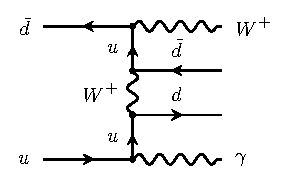
\includegraphics[width=\textwidth]{plots/diffx/vbswgEW1.pdf}
    \caption{}
\end{subfigure}
\hfill
\begin{subfigure}[b]{0.32\textwidth}
    \centering
    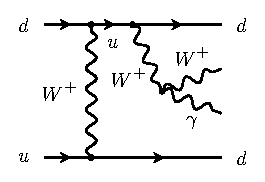
\includegraphics[width=\textwidth]{plots/diffx/vbswgEW2.pdf}
    \caption{}
\end{subfigure}
\hfill
\begin{subfigure}[b]{0.32\textwidth}
    \centering
    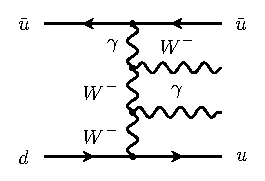
\includegraphics[width=\textwidth]{plots/diffx/vbswgEW4-1.pdf}
    \caption{}
\end{subfigure}
\hfill
\begin{subfigure}[b]{0.32\textwidth}
    \centering
    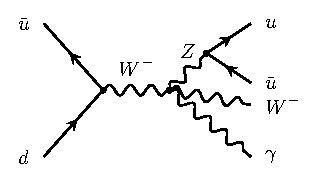
\includegraphics[width=\textwidth]{plots/diffx/vbswgEW5-1.pdf}
    \caption{}
\end{subfigure}
\hfill
\begin{subfigure}[b]{0.32\textwidth}
    \centering
    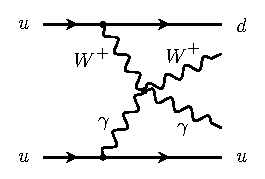
\includegraphics[width=\textwidth]{plots/diffx/vbswgEW3.pdf}
    \caption{}
\end{subfigure}
\hfill
\begin{subfigure}[b]{0.32\textwidth}
    \centering
    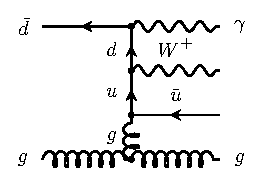
\includegraphics[width=\textwidth]{plots/diffx/vbswgQcd.pdf}
    \caption{}
\end{subfigure}
\caption{(a) \ewwy production involving no gauge boson self-interactions; (b) bremsstrahlung \ewwy non-VBS production involving trilinear gauge boson interactions; (c) \ewwy VBS involving trilinear gauge boson interactions; (d) \ewwy non-VBS production through s-channel triboson interaction involving EW quartic gauge boson interactions; (e) \ewwy VBS involving quartic gauge boson interactions; (f) \qcdwy production. Diagrams produced by author apart from (b) and (e), which are from \cite{VBSWy:VBSWy}.\label{fig:vbswy:diagrams}}
\end{figure}

\subsubsection{Status of VBS Measurements at ATLAS}

A summary of the standard model fiducial and total cross-section measurements derived at ATLAS are shown in Figure \ref{fig:smxsections}. From this figure it is clear that the VBS and VBF measurements correspond to some of the rarest standard model processes measured at ATLAS. In addition to electroweak $W\gamma jj$, some of the most recent VBS-sensitive measurements include 
\begin{itemize}
    \item The fidual cross-section measurement and observation of electroweak $W^{\pm}W^{\mp}jj$ production \cite{Theory:opsignww};
    \item The electroweak and inclusive differential cross-section measurements of $W^{\pm}W{\pm}jj$ production \cite{Theory:samesignww};
    \item Electroweak and inclusive differential cross-section measurements of $ZZ(\rightarrow4\ell)jj$ \cite{Theory:zzfourl}.
\end{itemize}
A summary of all public VBF, VBS, and triboson cross-section measurements, and their agreement with theory are shown in Figure \ref{fig:smvbsmeasurements}.

\begin{figure}
    \centering
    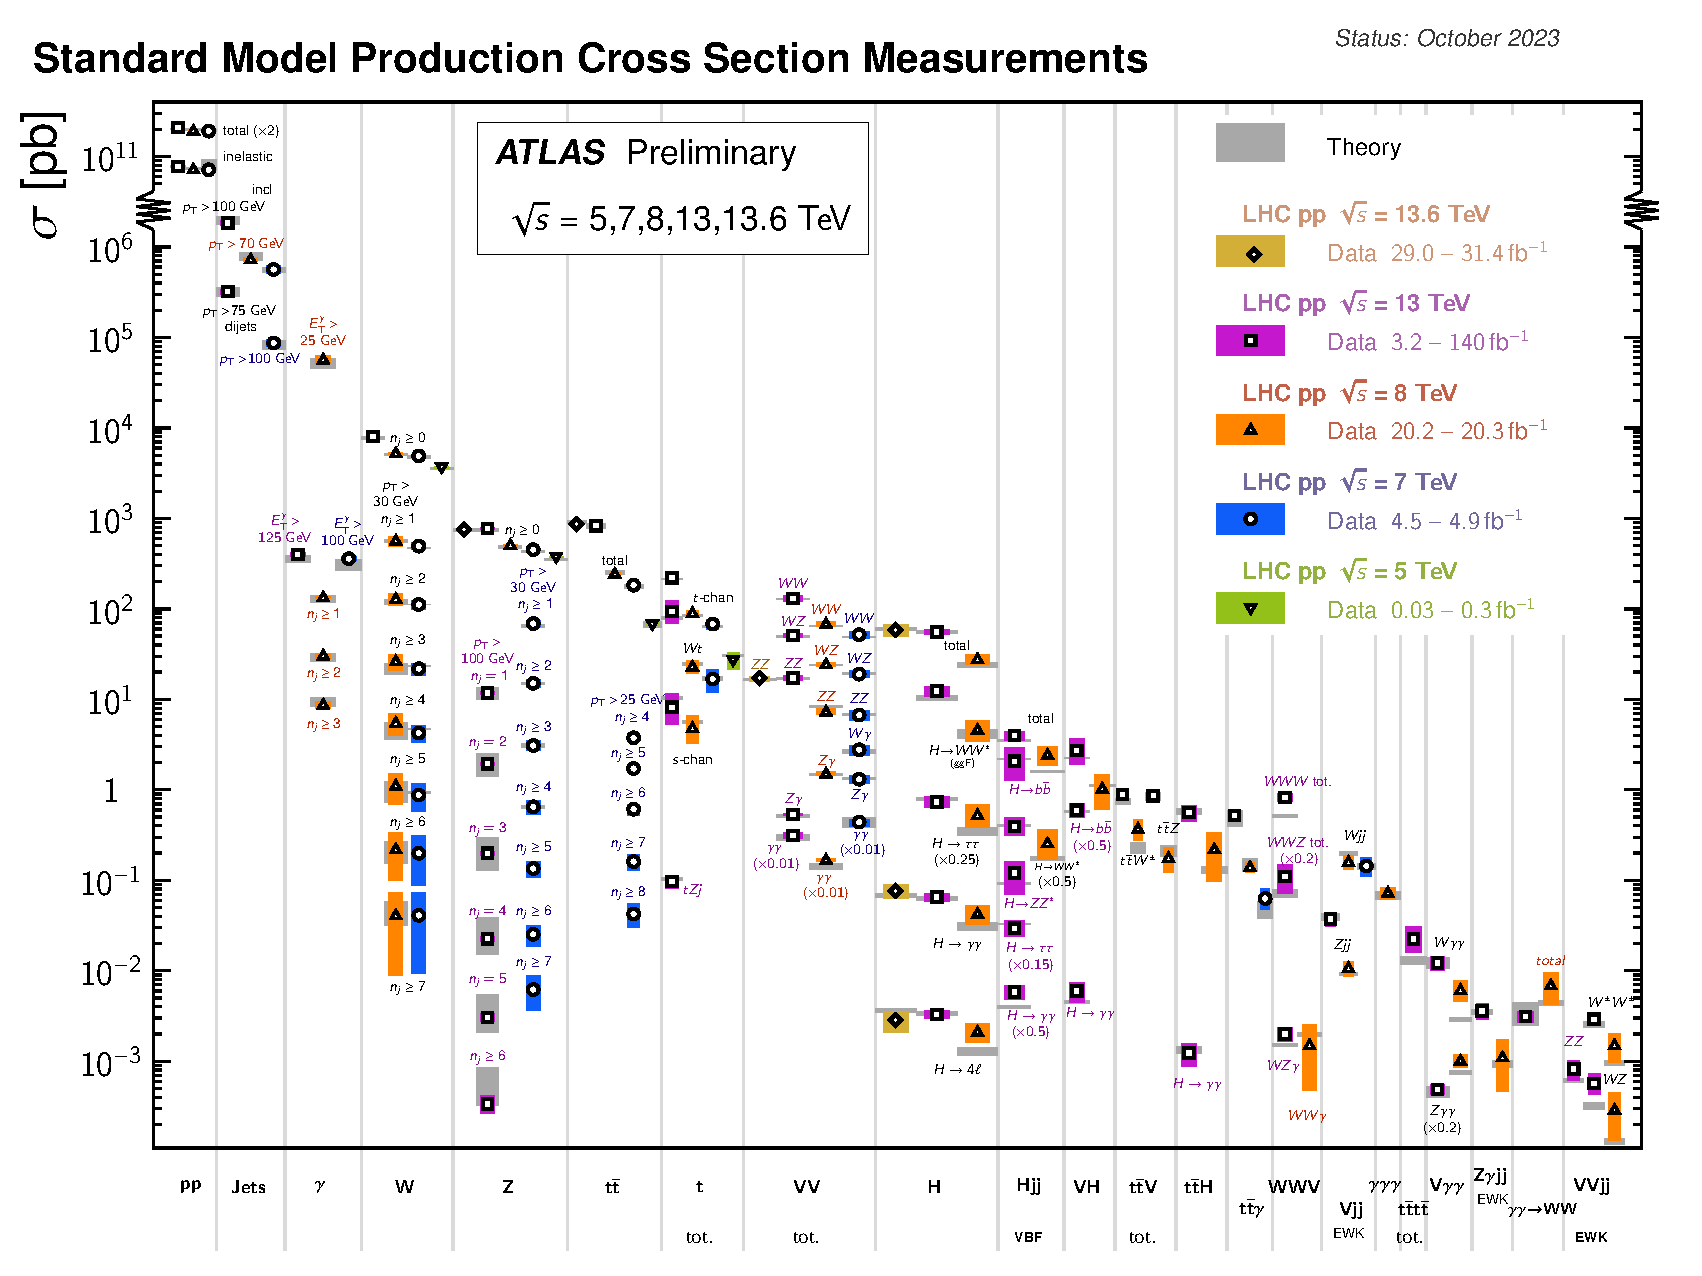
\includegraphics[width=\textwidth]{plots/theory/SM_summary_xsections.pdf}
    \caption{Overview of standard model total and fiducial cross-section measurements made at ATLAS. Total cross-sections are corrected for branching fractions. Figure from \cite{Theory:AtlasSummary}.\label{fig:smxsections}}
\end{figure}

\begin{figure}
    \centering
    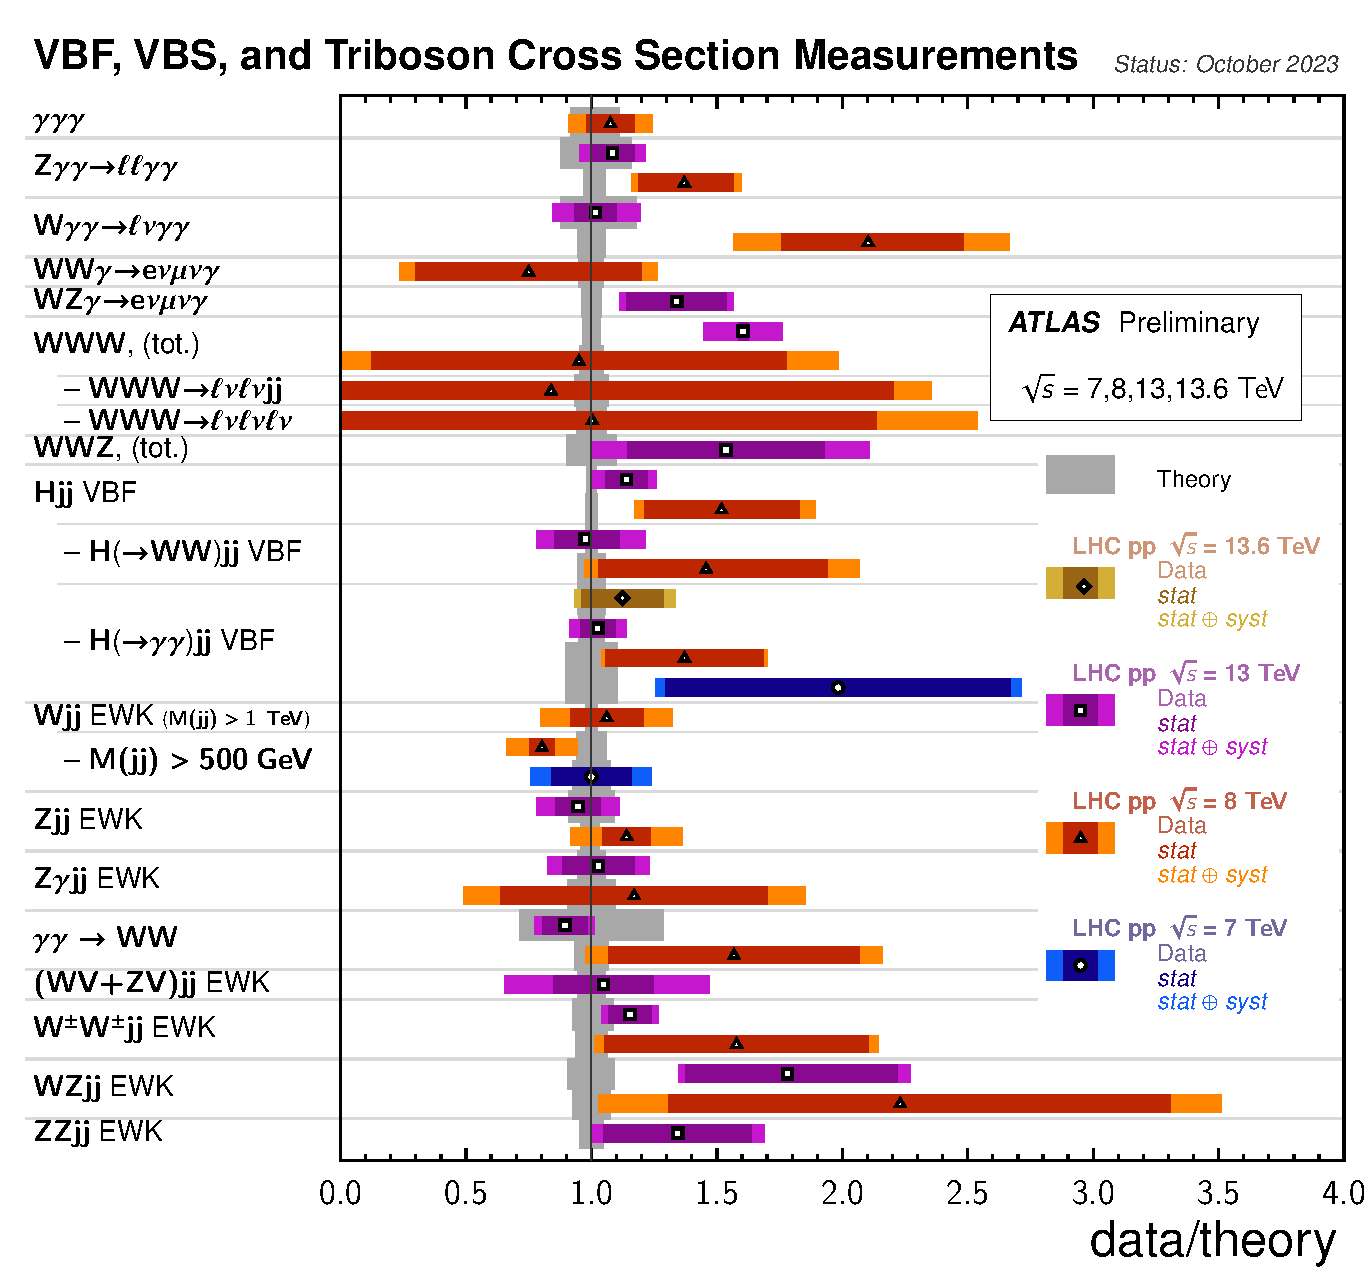
\includegraphics[width=\textwidth]{plots/theory/SM_VBS_Measurements.pdf}
    \caption{Overview data-to-theory ratios for a selection of ATLAS cross-section measurements for VBS, VBF, and triboson production. Measurements of these processes gives rise to an increasingly large body of constraints to quartic electroweak interactions. Figure from \cite{Theory:AtlasSummary}.\label{fig:smvbsmeasurements}}
\end{figure}

% Next status of VBS measurements and observations, and why background large, reword beginning a little bit

%Why backgrounds so much larger? Why large separation, tag jets etc.

% NEW SECTION -- VBS
% What is VBS? Why is it interesting? The Higgs divergence thing is of historical interest, can mention it but don't go into too much detail. Feynman diagrams, explain what's going in them and specifically using wyjj as an example and show the Wyjj (forward reference) diagrams to explain this. Then need a statement on what the backgrounds are [for wyjj I guess] and explain why the backgrounds are so much larger. Then describe the status of VBS measurements and observations at the LHC [can show the public cross-sections plot here if you want]. In general explain why VBS-weak boson self interactions are interesting. [A nice example from VBF higgs to show why the tagging jets appear: https://arxiv.org/pdf/1610.08420.pdf page 6]

%Something very quick about phase-space integrals (1-2 lines). Some 1-2 lines about differential cross-sections. Look for a bit to see if you can find an explicit example relating the VBS/VBF. Then go to PDFs

% Something about quanitising the above to get creation and annihilation operators -- still not sure if I actually needed to show the above. What are the states of the free hamiltonian, introduce free and interacting hamiltonian, interaction picture, time evolution operator.

%Plane wave solutions to the KG equation. After quantising can write scalar field operator in terms of anihilation and creation operators. Probability of a transition from state i to state j is given by PCP-2.109. Calculate inner product by S-matrix element.
% S-matrix element (or just matrix element) is the inner product of two states at times +/- infinity where the state at -infinity is evolved to +infinity by the operator S-operator in the interaction picture. David tong p54. PCP has a good discussion of this as well as QFT notes on page 62. [To calculate matrix element to first order, write initial and final states as anihilation and creation operators acting on the vacuum state, expand Shat in terms of powers of g (to first order), write the fields in terms of their creation and anihilation operators then use the ETCR to evaluate vevs of anihilation and creation operators]. We define the AMPLITUDE using equation (2.116, page57) of PCP (actually page 98 of QFT notes better). Can relate matrix elements to greens functions according to equation (18) -- qftmatrixtogreenfunctions.pdf handout -- where the green functions are the time-ordered vevs of fields with an shat operator. Then we can expand s-hat in terms of the interaction hamiltonian (page 80 of QFT notes) up to a given order. Can use wicks theorem to evaluate contractions etc, each contraction is a feynman propagator (scalar yukawa theory). Matrix elements can be represented by feynman diagrams using the feynman rules and where each distinct numerical contributions to a green's function corresponds toa single distinct feynman diagram. (FDs describe MEs not greens functions, AFIK the greens functions give the internal legs and vertices.. but it is still true that each contribution to a greens function has a single distinct feynman diagram -- double check definition of FDs with other sources). PCP - each feynman diagran is a precise mathematical contribution to the amplitude. From FD - xsections: 
% Go back to PCP-2.109, motivate the equation PCP-2.120 eventually giving 2.125-2.126. 

% 1. First subsection on scattering amplitudes and cross-sections. Relate scattering amplitudes to feynman diagrams and feynman diagrams to cross-sections. What is the partonic cross-section model. The thing that's calculable in perturbation theory. Start off with partonic cross-sections. Define interactions that lead you to cross-section. 
% 2. Bring in PDFs. These allow us to calculate cross-sections for processes in pp collisions. Then talk about how partons in final state will form hadronic systems -- The parton shower is/are an approximation to this. Perturbation theory is used, typically at NLO accuracy, sometimes only leading order. 
% 3. Hadronisation part (call this ``formation of hadronic final states'') -- ``catch-22 situation'' Andy suggested looking at how others resolve this...  Concept of PS is more a MC method. Parton shower -- [describes the?] dominant physics process. The ME diverges at small angles, this is the origin of parton shower. Not too many details on how hadronisation works. Should describe how to get from collisions to a stream of partons to hadrons. Should describe the divergence in the matrix element -- high virtuality -- [makes the final states?] likely to split into multiple partons.
% 4. Subsection on MC. (around 2 pages?) Partonic cross-section calculation at NLO using: [multiplicity??] merging, parton shower and hadronisation algorithms, underlying event and MPI. Then discuss what the state of the art in simulation is. Should discuss PS and hadronisation as a concept [I guess in the previous subsection] and then here go into the algorithms for the PS and hadronisation models e.g. PT ordering/angular ordering in pythia/herwig etc. 


%have an idential yukawa term as for leptons. eqn 4.6.17 with masses given by y_{u/d}v/sqrt(2). Here, just like in equation 2.46, we have assumed there are only diagonal yukawa terms, i.e. we don't have terms like y(l1phil2) [or can write q here]. However, in reality the matrix of yukawa terms only becomes diagonal by redifining the (lepton/) quark fields using  (eq 4.6.16), in this way V_6daggerYV is diagonal (this is called singular value decomposition). This rotation effects the kinetic term because left and right handed quark fields are rotated differently  resulting in terms like (eq 4.6.12), which implies that the weak interaction can change the quark family. This is summarised by the CKM matrix (eq 4.6.19). SSB gives rise to the quark mass terms, where the masses are given by (4.6.21). Finally can write down SM lagrangian.

%Now can have this bit in this section:  
%The SM has SU(3)xSU(2)xU(1) gauge symmetry, where the SU(3) gauge fields are given by G_munu. The residual symmetry group of the SM is SU(3)xU(1) (where the residual U(1) symmetry is actually a linear combination of original U(1) and a subgroup of SU(2)), meaning that SU(3) is not a broken gauge symmetry hence the G gauge fields do not gain mass under the higgs mechanism. Only a kinetic term for the G gauge fields. Therefore the covariant derivative term can be written like this: equation 4.5.1, where Y is the U(1) ``hypercharge'' which is just a real coefficient which changes depending on how a particular field transforms under U(1). The theory also contains a left-handed lepton field which has zero ``charge'' under SU(3) as leptons do not interact with the strong force and is doublet (for electron and neutrinos) (Write this down in the notation with three indices for the three different families). Since the weak force can change electrons into neutrinos they should be charged under SU(2) and since these are doublets they should tranform under the 2x2 matrices which make up the ``fundamental representation'' of SU(2) (rather than a different reducible representatoin which is not necessarily 2x2 matrices). We want the higgs field to be of the form discussed in the previous section, hence the hypercharge is 1/2 and should have SU(3) charge of zero. The theory also contains a one-component right handed spinor field which is neutral (uncharged) under SU(3) and SU(2). Go over charge operator and why hypercharges have to be -1/2 and -1. Mass term like equation (4.5.9) is not allowed, therefore write it like (4.5.10) and now this is invariant under SU(2) and U(1). After SSB becomes (4.5.17) and the left and right handed spinors have combined to become the physical electrically charged lepton fields. No mass term for neutrinos. Masses are given by ml^f = y_l^fv/sqrt(2). 


% Note to self: Probs too much info, but the A_mu gauge field components here are in the T-hat basis, so the eigenvectors of the S_ab matrix give the combinations of the A_mu in the original basis, the components of these eigenvectors are the cos and sin weinberg angles. Also for the W boson we can express these as 1/sqrt(2)(A^2\pmiA^3) because in the quadratic part of the lagrangian we have 0.5Amu^2Amu^2 + 0.5Amu^2Amu^3 + ... but this is equivalent to 1/2(amu^2\mp iamu^3)(amu^2\pm iamu3) which can then be identified as the W boson fields. So, tldr - what I wrote above is correct. 
%\begin{equation}
%    
%\end{equation}
% To realise the lagrangian for the unified electroweak theory, have to introduce the concept of local non-abelian gauge transformations, in this case a scalar field transforms as phi->matrix phi, and vector field as A-> MAMdagger + ... . The special unitary group SU(N ), defined as the group of complex N × N matrices with M † M = 1 and det M = 1. Number of basis matrices -- generators -- given by D = N^2-1 (U(1) is D=N^2)``dimensionality of the group''. Non-abelian local gauge transformations can be realised if the gauge field can be written as a linear combination of the generators of the group (representation). (we say the gauge field is an element of the algebra). This means the gauge fuield can be written as a D component vector field. Write A^mu in terms of generators. Using this notation, it is useful to define the matrix Sab. Can show that the unbroken generators are giben by eigenvectors of Sab with zero eigenvalue. The eigenvectors of Sab can be used to define a new set of generators ordered such that the broken generators come first. (since the unbroken generators leave the vev unchanged, these generate the ``residual symmetry group''). 
% The most general lagrangian in scalar field theory is dmuphidmuphi - potential, dmuphidmuphi is the kinetic term. The kinetic term for the gauge field lagrangian (fmunufmunu) is not gauge invariant in the non-abelian case. However, can show that the TRACE is invariant. Therefore can write down a lagrangian invariant under local U(1) and (non-abelian) SU(2) transformations as [Lagrangian on page for of SM_mccullough], where for the kinetic term of the scalar field, we have covariant derivatives since we have gauged the symmetry (since lagrangian invariant under LOCAL gauge transformations). Now can go into EW unification.
% Consider lagrangian EW unification lagrangian from mccullough (where Amu = Amu^at^a), this has SU2 x U1 symmtery. dimensionality of SU2 is three, therefore there are three SU2 gauge fields (A_mu^a), U(1) has dimensionality one therefore one U(1) gauge field, B_mu. Now, rewrite covariant derivative as in (3.7.4), now can write (Dmuphi)_i as equation 3.6.2, where phi^hat = blablabla. Using that fact phihatphihat = lambda^Bdelta_ab (equation 3.6.4), can write the covariant derivative term as equation (3.6.5) (to quadratic order). Cannot identify mass because of the mixing term. Can remove this mixing term through a gauge choice -- unitary gauge -- which is defined by (equation 3.6.12 with mij replace with 2lambda v^2). Mass of the scalar particle is sqrt(2lambda) v and the eigenvalues of the S matrix give the masses of the vector particles. Now write down Sab as equation (3.7.6), introduce weinberg angles etc, use the pauli matrices and give the eigenvalues and therefore that masses of the photon, W+- and the Z.  
%Only considered Abelian case thus far. (higgs vev 246 GeV)

% adding interaction term is equivalent to ``gauging the symmetry, which is replacing derivatives with covariant derivatives turning the global u(1) symmetry into a local symmetry. ''
%%%%%%%%%%%%%%%%%
%* Say a little bit about local symmetries, (gauging the symmerty?).
%* Motivation (no quite a derivation) of Maxwell lagrangian describing the (massless) photon as a (spin-1) vector field which reproduces all of Maxwell's equations but with zero charge(density) and no current(density) term. Gauge transformations: different vector and scalar potentials give rise to the same electric and magnetic field, so we are free to impose invariance under these transformations. Maxwell Lagrangian Doesn't describe interactions, doesn't describe electrons.Amu = (A,phi). EoM give spatial components satisfy massless Klein-Gordon equation after choosing the ``radiation gauge''. Gauge invariance gives masslessness of photon 
%* Have talk about noninteracting photons, for description of electrons discuss Dirac equation, spinors, spin, etc. Dirac lagrangian. Global U(1) symmetry gives rise to the conserved noether current $j^mu$. Mention Noethers theory says that symmetries give rise to conserved currents. After the spinors are quantised, this leads to a conserved noether charge of PS9[3.113] (page62) which gives the number operators for particle and antiparticles with charge -e. Dont even need to mention raising and lowering operators, just use number operator. Next, gauging the symmetry gives rise to interactions between photons and electrons. Then have the full QED |Lagrangian. 
%Spinors tranform differently than vectors under lorentz transformations

%describes a fixed number of particles %the state of the system is described by a wave function $\psi(x)$.
%\begin{equation}
%    \langle\psi,\phi\rangle=\int\mathrm{d}^3x\psi^*(\underline{x}\phi(\underline{x}))
%\end{equation}
%QM describes a fixed number of particles (or a single particle).
%The basic structure of QM persists to all generalisations such as QFT, string theory, ... No evidence against the basic mathematical structure of QM. 
%QM assumes the universe is split into quantum and classical regimes (unsatifactory)
%
%
%Introduce Theory
%
%\section{QFT and the Standard Model}
%\subsection{Classical Field Theory}
%* Scalar and Vector Fields \\
%* The Maxwell Lagrangian \\
%\subsection{Symmetries in Field Theory}
%* Abelian and non-Abelian Symmetries \\
%* Symmetry groups and Lie Algebras \\
%* Noether's theorem \\
%* Non-Abelian Gauge Fields \\
%* Spontaneous Symmetry Breaking \\
%* (non-Abelian) Higgs Mechanism \\
%* EW Symmetry Breaking \\
%\subsection{Fermions}
%* Dirac Equation \\
%* Dirac Lagrangian \\
%* Leptons \\
%* Quarks \\
%\subsection{The Standard Model}
%\subsection{Calculation of Cross Sections}
%* Phase space integrals \\
%* Example in QED \\
%\subsection{Effective Field Theories}
%\section{Collider Phenomenology and MC generators}
%\subsection{Basics of non-perturbative QCD}
%* Infrared, collinear divergences, IRC safety \\
%* IR limits and ME factorisation \\
%* parton showers, hadronisation, different hadronisation models  \\
%* Resummation  \\
%* Deep inelastic scattering, PDFs \\
%\subsection{Jet Clustering and Jet Substructure}\label{sec:theory:jet}
%* Jet Algorithms \\
%* Cone Algorithms \\
%* Sequential Recombination Algorithms \\
%* Jet Input Objects and Jet Tagging \\
%\subsection{Event Generators}
%* Basics of Monte Carlo methods \\
%* Non-perturbative QCD in MC generators \\
%* Multi-parton interactions, pile-up \\
%* Overview of different MC generators (e.g MG5 vs Powheg vs Sherpa), differences between them, assumptions made \\
%\section{Physics of Vector Boson Scattering/Fusion}
%* Typical event topology and relation to colour flow \\
%* Typical observables characterising VBS/VBF processes \\
%* EFTs and sensitivity to Dim-6 and Dim-8 operators \\
%* CP-odd observables
%